\documentclass[11pt]{article}
\usepackage[utf8]{inputenc}
\usepackage{graphicx}
\usepackage[ngerman]{babel}
\usepackage{url}
\usepackage{float}
\usepackage[backend=bibtex,style=alphabetic,sorting=ynt]{biblatex}
\usepackage[dvipsnames]{xcolor}
\usepackage[left=3.5cm, right=2.5cm, top=2.5cm, bottom=2cm]{geometry}
\addbibresource{literatur.bib}
\graphicspath{ {./images/} }
\title{
{Construction and Validation of a Guideline for migrating a Microservice Architecture to Function as a Service}\\
{\large Frankfurt University of Applied Sciences}\\}
\author{Gianni Pasqual}
\date{18.03.2020}
\begin{document}
\maketitle
\newpage
{\Large \textbf {Abstract}}
\\\\
Mit der Technologie Function as a Service ist nach der Microservice-Architektur eine noch feinere Modularisierungsstufe von Software erreicht worden. Mit dieser ist es möglich Software noch schneller bereitzustellen und im gleichen Zuge Einsparungen bei dem Betrieb der IT-Infrastruktur zu erzeielen. Dies erscheint auf den ersten Blick natürlich sehr lokrativ für viele Unternehmen, jedoch sollte die Entscheidung für den teilweisen oder gesamten Umzug der Service-Landschaft wohl überlegt sein. Wie bei jeder anderen Technologie hat auch diese ihre Potentiale und Herausforderungen die gemeistert werden müssen. Für Unternehemn, die sich dazu entschieden haben Function as a Service (FaaS) in ihre Infrastruktur einzubinden, soll diese Arbeit als Orientierung bei der Migration dienen. Da viele Unternehmen bereits von den monolithischen Anwendungen auf kleinere modularere Services umgestiegen sind, geht diese Arbeit von einer bereits vorliegenden Microserive-Architektur aus. Es gilt herauszufinden in welchem Maße und ob überhaupt strukturelle Anpassungen vorgenommen werden müssen, als auch der Frage nach "Best-Practices", nach nun knapp vier Jahren des Bestehens, nachzugehen.
\\\\
Zudem soll sich vor allem mit dem von den verschiedenen Anbietern ausgehenden Vendor-Lock-In auseinadner gesetzt werden und erarbeitet werden, welche Möglichkeiten bestehen, diesen zu umgehen bzw. zu mildern. Um mögliche Schwächen des Leitfadens aufzuzeigen, soll dieser beispielhaft an einem Service erprobt werden und auftretenden Fehler dokumentiert und behandelt werden.
\newpage
{\Large \textbf {Index of abbreviations}}
\\\\\\
\begin{tabular}{ p{2cm} p{10cm}} 
ADF & Azure Durable Functions \\
API & Application Programming Interface \\
ASF & Amazon Step Functions \\
AWS & Amazon Web Services \\
BaaS & Backend as a Service \\
BDD & Behaviour Driven Development \\
CaaS & Container as a Service \\  
CD & Continuous Delivery \\  
CI & Continuous Integration \\
CLI & Command Line Interface \\
CNCF & Cloud Native Computing Foundatino \\
CPU & Central Processing Unit \\
CRD & Custom Resource Definition \\
DevOps & Development and Operations \\  
DEV & Development \\
DSL & Domain Specific Language \\
FaaS & Function as a Service \\ 
HPA & Horizontal Pod Autoscaler \\
IAM & Identity Access Management \\
IaaS & Infrastructure as a Service \\
IaC & Infrastructure as Code \\
INT & Integration (Testing) \\
IT & Information Technology \\
JVM & Java Virtual Machine \\
NIST & National Institute of Standards and Technology \\
OOP & Object Oriented Progamming \\
OS & Operating System \\
PaaS & Platform as a Service \\
POM & Project Object Model \\
PR & Pull Request \\
PRD & Production (Environment) \\
RPC & Remote Procedure Call \\
SAM & Serverless Application Model \\
SDK & Software Development Kit \\
UAT & User-Acceptance (Testing) \\
VCS & Version Controle System \\
XaaS & Anything as a Service \\
\end{tabular}
\newpage
\tableofcontents
\newpage
\section{Einleitung}
\subsection{Forschungsfrage und Ziele der Arbeit}
\subsection{Erläuterung der Problemstellung}
\subsection{Aufbau der Thesis}










\section{Aufarbeitung des Themengebietes}
Ist eine Technologie, wie Function as a Service, noch relativ jung, so sind die Schritte der Findung einer in sich schlüssigen und allgemein vertretenen Definition oftmals noch nicht abgeschlossen. Auch bei der Definition von FaaS, Serverless und der Einordung dieser beiden Konzepte in die Infrastruktur des Cloud Computings8  \cite{mell2011nist}, ist dieser Prozess noch im Gange, wobei mitlerweile die unterschiedlichen Definitionen der offentlichen FaaS- und Serverless-Anbieter einige Gemeinsamkeiten aufweisen. Trotz alledem bestehen weiterhin Ungenauigkeiten, die es in den nächsten Jahren noch zu beseitigen gilt. Hierzu später mehr.\\\\


\subsection{Definition des Begriffes Cloud Computing}
Der Begriff Cloud Computing ist laut eines Technology Report bis auf das Jahr 1996 zurückzuführen, wo er in einem Business-Plan des Unternehmens Compaq von ein paar Entwicklern genutzt worden sein sollen, um über die zukünftigen Entwicklungen des Internet-Businesses zu diskutieren \cite{regalado2011coined}.\\\\
Auch wenn das Konzept des Cloud-Computings, die dynamische, skalierbare, zuverlässige und unbegrenzte Bereitstellung von Ressourcen als Dienst über das Internet, immer mal wieder in der Literatur auftauchte \cite{fox2009above}, so erlangte es erst ab 2006 einen immer größter werdenden Bekanntheitsgrad. 2006 veröffentlichte AWS das Produkt Elastic Compute Cloud (EC2), gefolgt von Goolges App Engine 2008. Bereits in diesem früher Stadium wurde mit App Engine das Prinzip einer sog. \glqq stateful\grqq{}-Ebene, für das Speichern von des Aktuellen Anwendungsstatus und einer \glqq stateless\grqq{}-Ebene für die Ausführung des eigentlichen Programmes unterschieden \cite{fox2009above}. Des Weiteren wurde 2009 in einer Berkeley-Studie die sechs größten Potentiale des Cloud-Computings herausgearbeitet welche bis heute in den unterscheidlichen XaaS-Konzepten umgesetzt wurden. Im folgenden sind diese kurz auf gelistet. \\
\begin{itemize}
\item[1.] Unbegrenzte Ressourcen wann immer sie benötgt werden. 
\item[2.] Durch die Möglichkeit mit wenigen Ressourcen zu starten, vielen Nutzern zugang zu der Plattform zu gewähren. 
\item[3.] Die genutzen Ressourcen so genau wie möglich nach dem \glqq Pay Per Use\grqq{}-Prinzip zu bezahlen. 
\item[4.] Größenvorteile (Economies of scale) nutzen, um die Kosten durch eine dauerhafte, optimale Ausnutzung riesiger Datencenter auf ein Minimum zu reduzieren. 
\item[5.] Operationelle Kosten so weit es geht zu senken und die Ressourcennutzung durch Virtualisierung so weit wie möglich auszunutzen. 
\item[6.] Eine hohe Hardwareausnutzung durch \glqq Multiplexing\grqq{} der Auslastungen verschiedener Unternehmen zu erreichen.
\end{itemize}
Das National Institute of Standards and Technology (NIST) veröffentlichte 2011, nach 16 vorausgehenden Definitionen, schließlich eine finale Definition des Cloud-Computings, welche bis heute als orientierung Anwendung findet und in einer vielzahl an Werken aufgegriffen wird \cite{mell2011nist}. Die Definition nach NIST beschreibt das Cloud model als eines aus fünf essentiellen Charakteristiken und drei Service Modellen, IaaS, PaaS und SaaS bestehendes Modell, mit insgesamt vier Deployment-Models.\\\\
\textit{"Cloud Computing is a model for enabling ubiquitous, convenient, on-demand network access to a shared pool of configurable computing resources (e.g., networks, servers, storage, applications, and services) that can be rapidly provisioned and released with minimal management effort or service provider interaction."} \cite{mell2011nist}.\\\\
NIST bricht die Definition mit Essentiellen Charakteristiken, Service-Models und Deployment-Models in drei Unterkategorien herunter, welche erfüllt sein müssen um dem Anspruch an Cloud Computing zu genügen. \\
Grob gefasst sind dies bei den Characteristiken, die automatische Bereitstellung der benötigten Ressourcen je nach bedarf (\textit{On-demand self-service}), die Möglichkeit von allen gängigen Geräten darauf zugreifen zu können (\textit{Broad network access}), die optimale Verteilung von Ressourcen auf die Kunden welche sie gerade benötigen, wobei hier die exakte lokation dieser von geringer Relevanz ist (\textit{Resource pooling}), die automatische Skalierung von Ressourcen (\textit{Rapid elasticity}) und die Möglichkeit der Überwachung und Limitierung der Ressourcenausnutzung, welche für den Kunden als auch den Anbieter transparent sein muss (\textit{Measured service}).\\\\
Bei den Service Models werden hier lediglich IaaS, PaaS und SaaS unterschieden. Laut NIST gibt es um den Code in der Could bereitzustellen vier verschiedene Deployment-Models, welche genutzt werden können. Mit der \textit{Private cloud}, obliegt es dem Unternehmen seine Infrastruktur komplett selber zu betreiben, jedoch muss diese dem Unternehmen dabei nicht selber gehören, sondern kann von eine dritten Partei gehostet werden. Mit dem deployment auf eine \textit{Community cloud} teilen sich verschiedene Unternehemen eine Cloud, welche entweder von ihnen gemeinsm, oder von einem Drittanbieter betrieben wird. Zuletzt gibt es noch die Möglichkeit die von einem Cloud-Computing-Anbieter bereitgestellte öffentliche Cloud \textit{Public cloud} zu nutzen, bei welcher das Unternhemen die Räumlichkeiten bzw. Ressourcen von einem Dittanbieter nutzt. Das letzt Deployment-Model stellt die sog. \textit{Hybird cloud} dar, welche eine Kombination aus den vorherigen darstellt \cite{mell2011nist}.
\begin{figure}[H]
\caption{Übersicht Service-Models Cloud-Computing}
\label{fig:cloudComputingConcepts}
\centering
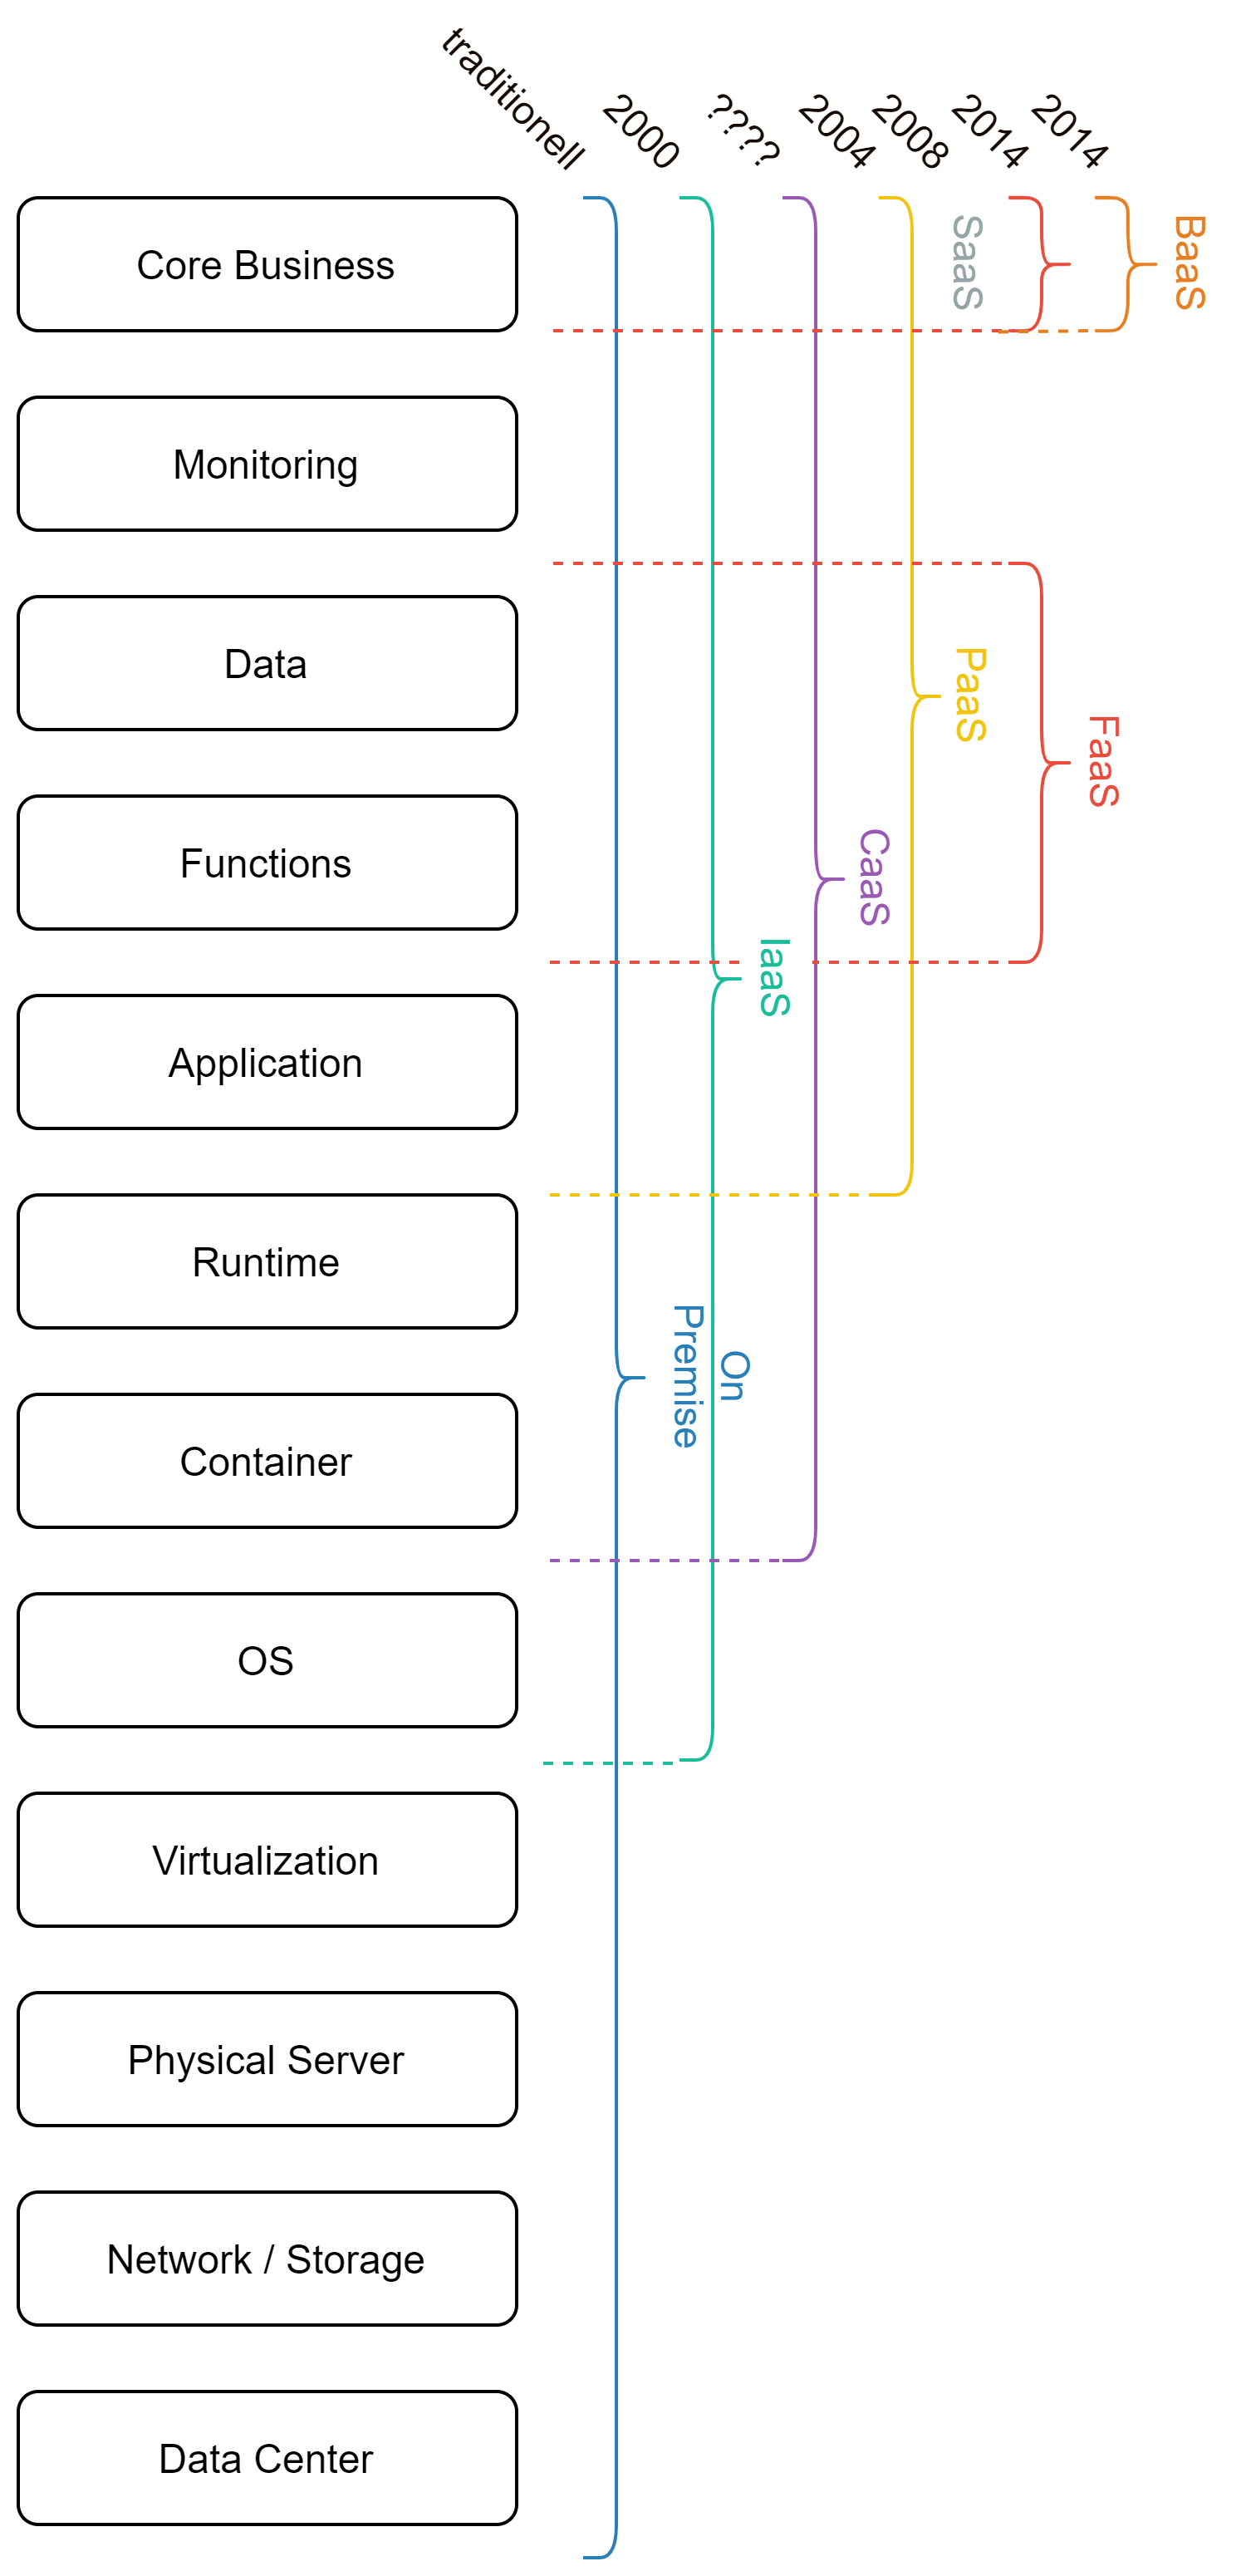
\includegraphics[angle=90,width=1\textwidth]{serviceModels}
\end{figure}
Neben den bereits genannten Service Models IaaS, PaaS und SaaS gibt es jedoch noch weitere, welche sich im Laufe der Zeit etabliert haben. Abbildung ~\ref{fig:cloudComputingConcepts} gibt einen Überblick hierüber. 


\subsection{Function as a Service}
Function as a Service (FaaS) ist ein sogenanntes \glqq Serverless\grqq{} Cloud-Computing Konzept, welches erstmals 2014 von AWS mit Lambda Functions als Preview Release und schließlich 2015 zur kommerziellen Nutzung zur Verfügung gestellt wurde\footnote{https://docs.aws.amazon.com/lambda/latest/dg/lambda-releases.html}. Es kann nach IaaS und PaaS als ein weiterer Schritt in der Entwicklung des Cloud Computings gesehen werden, welcher das Management von Infrastruktur, Servern und Ressourcen weg von dem Entwickler nimmt und hin zu dem Cloud-Anbieter delegiert. Ein knappes Jahr später, 2016, traten Microsoft mit Azure Functions, Google mit Google Cloud Functions und IBM mit OpenWhisk in den bis dahin von Amazon dominierten Markt ein. Mittlerweile gibt es eine vielzahl an Open-Source sowie proprietären Anbietern, welche um die Gunst der Kunden werben und einen stetigen Wettbewerb aufrecht erhalten. Ein ausführliche Übersicht über die jeweiligen Anbiter findet sich online von der CNCF\footnote{https://github.com/cncf/wg-serverless}\\\\
Da es sich mit FaaS und Serverless um eine noch recht junge Technologie handelt gibt es zu diesem Konzept keine offiziell dokumentierte Definition. bsp. von NIST o.ä., in der Literatur, wie es beispielsweise beim Cloud-Computing \cite{mell2011nist} der Fall ist. Die Anbieter sind sich jedoch über die Funkitionalität von FaaS größtenteils einig, was das Spektrum an Funktionalitäten anbegeht. So definiert Microsoft Azure Functions als: \glqq [...] event-driven serverless compute platform that can also solve complex orchestration problems. Build and debug locally without additional setup, deploy and operate at scale in the cloud, and integrate services using triggers and bindings. \grqq{}\footnote{https://azure.microsoft.com/en-us/services/functions/}. Hiermit beschreibt der Anbieter bereits die Kernfunktionalitäten von FaaS und drückt den Kerngedanken hinder FaaS aus. Das Konzept soll genutzt werden können, um bei dem Auftreten eines zuvor definierten sog. Triggers auf ein Event aus der eigenen Applikation oder der des Abieters reagieren zu können. Dabei stellen die meisten Anbieter wie Google, Azure oder AWS neben einem einfachen event-basierten HTTP-Trigger oder widerkehrenden zeitbasierten Triggern noch weitere, an die jeweilige Infrasturktur des Anbieters angepasste, Trigger zur Verfügung. Diese ergeben sich meist aus den BaaS Angeboten, hierzu mehr in \textit{Abgrenzung von FaaS zu Serverless}, welche in Form von Datenbank Triggern bei einer CRUD-Operation, dem Anlegen eines Nutzers oder der Integration mit einem Push-Notification Service [AWS SSN, Google Pub/Sub etc.] auftreten können.\\
\begin{figure}[H]
\caption[FaaS Programming Model nach OpenWhisk]{\footnote{http://openwhisk.apache.org/documentation.html}}
\label{fig:openWhiskProgrammingModel}
\centering
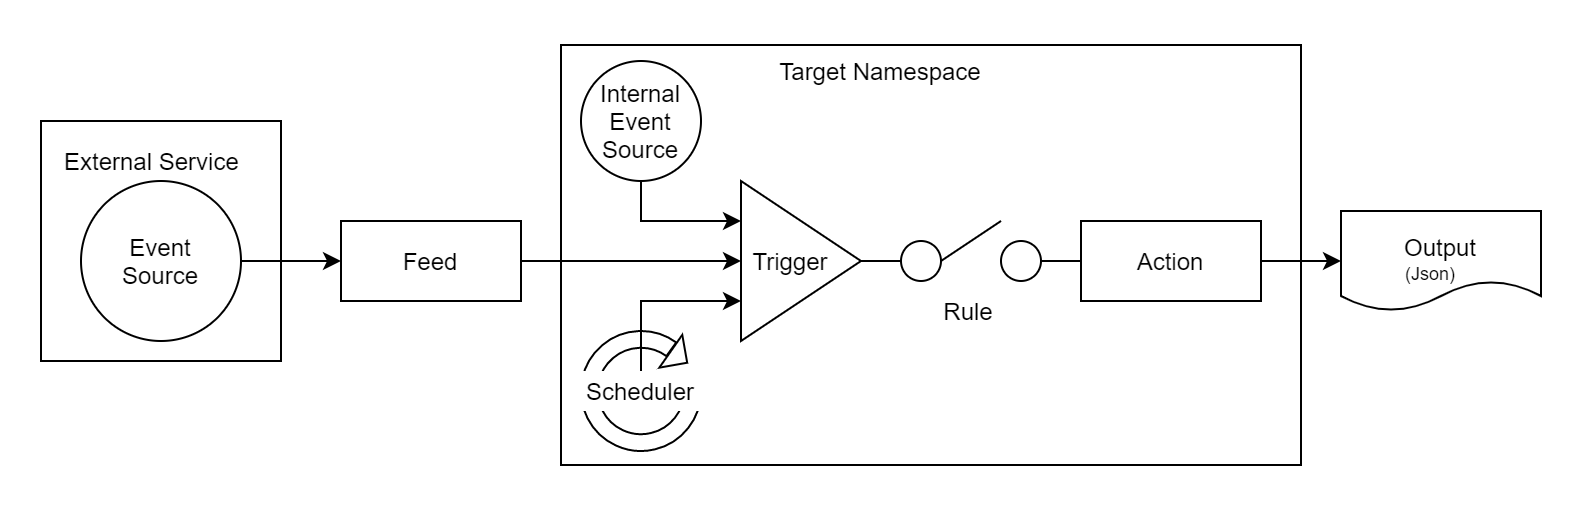
\includegraphics[width=1\textwidth]{ProgrammingModel}
\end{figure}
Abbildung ~\ref{fig:openWhiskProgrammingModel} gibt hierbei eine Übersicht über die verscheidenen Event-Trigger, welche derzeit bei den großen, proprietären Anbietern (AWS, Google, Microsoft) existieren. Da hinter OpenWhisk mit IBM eine großes Unternehmen steht, wird dieses Modell in der Literatur häufig als Referenz in Bezug auf die anderen Anbieter verwendet. Es kann angenommen werden, dass andere Abieter ein ähnliches Konzept bei ihrer FaaS Architektur verfolgen, da Apache OpenWhisk in einer großen Cloud (IBM) bereitgestellt wird \cite{van2019spec}. Eine weitere fundamentale Eigenschaft ist die erwähnte Skalierbarkeit, welche nach dem sog. \glqq Pay Per Use\grqq{}-Modell abgerechnet wird. Gemeint ist hiermit, dass der Kunde nur das bezahlt was er auch wirklich verbraucht hat, wobei die Verrechnung extrem granular nach genutzten Ressourcen und gelaufener Zeit erfolgt. Der Kunde bezahlt daher nicht für die benötgten Ressourcen, wie er es bei PaaS (wobei es hier variierende und bereits granularere Modell gibt) oder IaaS der Fall ist, sondern nur für die tatsächlich genutzten Ressourcen.\\\\
\textcolor{blue}{Grundsätzlich ist zwar der Preis der für das Laufen einer einminütigen Funktionsaussführung verglichen mit dem Laufen des selben Codes auf einem von den Ressourcen her ähnlich bestückten PaaS-Server günstiger \cite{jonas2019cloud}, jedoch der Anwendungszweck ein ganz anderer. Während mit PaaS Anwendungen bedient werden, die eine dauerhaft hohe Nachfrage erfahren, sollen mit Funktionen primär einfache stark frequentierende Aufgaben geläst werden, bei denen der Nutzer nur für die Ressroucen bezahlen muss die die Funktion bei dem Aufruf nutzt und nicht für jene die ohen einkommende Aufrufe provisioniert wurden.}\\\\
Ein weiterer wichtiger Punkt, welcher sich auch bei anderen Anbietern findet, ist in der Definition von OpenWhisk zum einen mit \glqq[...] you can focus on building amazing and efficient applications [...]\grqq{} und zum anderen mit \glqq  developers write functional logic [...] in any supported programming language, that can be dynamically scheduled [...]\grqq{}\footnote{http://openwhisk.apache.org/}. Ersteres meint die Abstraktion der Infrastruktur, welche dem Nutzer zum Bereitstellen von lauffähigem, skalierbaren, sicheren Backend-Code nicht bekannt sein muss. Die automatische Skalierung und optimale Verteilung von Ressourcen obliegt der Hoheit des Anbiters, und ist dem Nuzter nicht zugänglich, zumindest bei den proprietäre Anbietern. Letzteres ist zwar keine einzigartige Eigenschaft von FaaS, da dieses Konzept beriets lange bekannt ist und auch bei der Microservice-Enticklung häufig zum Einsatz kommt, jedoch ist die Auswahl aus vielen verschiedenen Programmiersprachen wie Java, Go, Javascript (Typescript), Python, PHP usw. (abhängig von dem jeweiligen Anbieter) unter dem Gesichtspunkt der direkten Nutzung zu sehen. Es muss keinerlei zusätzliches Setup oder andere Konfigurationen in der Umgebung vorgenommen werden, da dies der Anbieter übernimmt. Er kümmert sich um Patches und das Upgraden auf die aktuellste Version, was dem Entwickler ein großes Maß anflexibilität bei der Entwicklung der Anwendung einräumt. Eine weitere häufig in der Literatur referenzierte Defninition ist \cite{fowler2018serverless}, von Mike Roberts, welche die Beschreibung von AWS Lambda näher erläutert und im groben die oben genannten Punkte wiedergibt. \textcolor{blue}{Natürlich sind diese Eigenschaften mit einem gewissen Venodr Lock-In \textcolor{red}{dieser jedoch weder als schlecht noch gut zu bewerten ist und vielmehr nüchtern auf seine Vor- und Nachteile anasystiert werden sollte.} verbunden, da dieser Enstcheidungen über die Infrastruktur trifft, mehr dazu in \textit{Potentiale und Herausforderungen}.}\\\\
Abbildung ~\ref{fig:FaaSBaaSExample} verdeutlicht hierbei noch einmal die Wirkungsweise von FaaS. Oben rechts ist der Funktionspool zu sehen, welcher bei dem jeweiligen Cloud Provider steht und in welchen der Entwickler seine Funktionne lädt. Wird eine Funktion von einem Client aufgerufen, so wird bei Aktivierung eines Triggers eine Kopie der jeweiligen Funktion instantiiert und alle mit diese Funktion verbundenen Abhänigkeiten geladen (bspw. benötigte Module). Je nachdem wie frequentiert die Funktionen von den Clients angefordert werden, werden die vorhandenen Instanzen automatisch von dem Provider 
\begin{figure}[H]
\caption{Anwendung mit FaaS und (P)BaaS, angelehnt an \cite{shafiei2020serverless}}
\label{fig:FaaSBaaSExample}
\centering
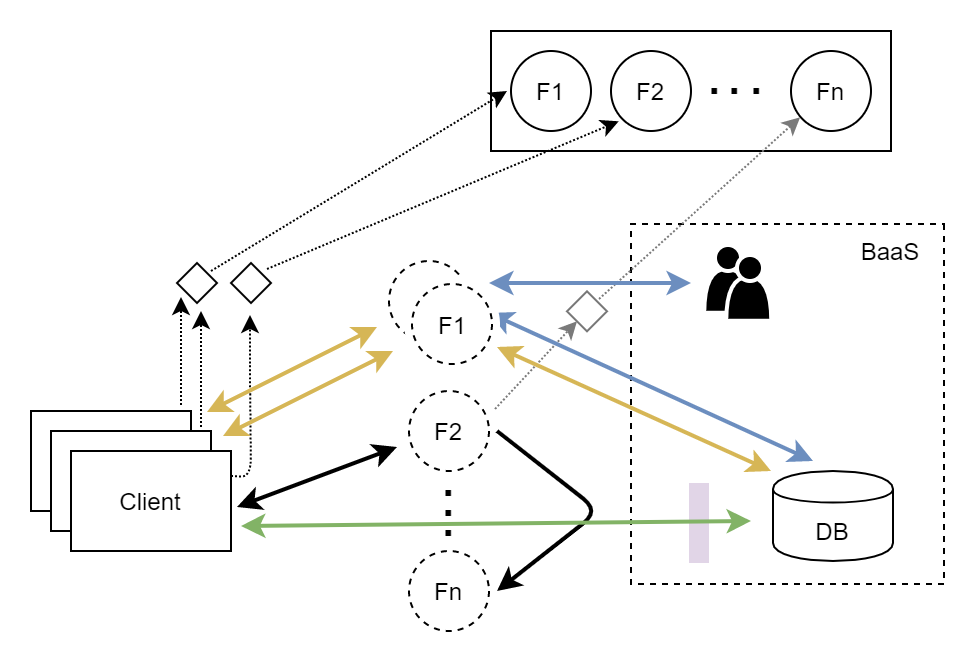
\includegraphics[width=0.7\textwidth]{FaaS}
\end{figure}
hochskaliert, um den eingehenden Anfragen gerecht zu werden. Hierbei kann die Funktion eine Aufgabe direkt ausführen und das Resultat an den Client zurückgeben, oder wie bei F1 auf die im hintergrund laufende BaaS Infrasturktur zugreifen. Diese reicht von einfachen Datenbankabfragen bis hin zu anlegen eines neuen Nutzers etc. Limitiert werden die Möglichkeiten hierbei lediglich von dem Service-Ökosystem des jeweiligen Anbieters. Genauso ist es natürlich möglich Funktionen sich gegenseitig aufrufen zu lassen oder direkt mit BaaS-Servicen zu interagieren, siehe \textit{Abgrenzung von FaaS zu Serverless}.\\\\
Um FaaS besser und einheitlicher definieren zu könne und damit einen plattformübergreifenden Standart zu schaffen, wird in der Industrie und Forschung das Verlangen nach einer Referenzarchitektur, wie sie beispielsweise für das Cloud oder Grid Computing vorhanden ist \cite{liu2011nist}, \cite{foster2003grid} lauter. Die Abwesenheit einer solchen Architektur behindere die Etablierung von Best-Practices, Design Pattern und einen genaueren Überblick darüber zu erhalten, wie sich das Feld rund um Function as a Service entwickele \cite{leitner2019mixed}. Erste Vorschläge wie die Referenzarchitektur von FaaS aussehen könnte, haben sich mit \cite{van2019spec} durch die über die Jahre, von 2016 an, gestiegenen Popularität von Faas in der Forschung und der Literatur bereits herausgebildet. War hier die Thematik bis 2016 nicht addressiert worden, so stieg die Präsenz von hier an kontinuierlich bis 2019, in Journals, Konferenzen und Workshops an \cite{Yussupov2019_SystematicMappingStudyFaaS}.\\\\


\subsection{Abgrenzung von FaaS zu Serverless}
Serverless-Computing, oftmals auch als Serverless bezeichnet, ist eine Teildisziplin des Cloud-Computings, welche sich aus der Virtualisierung von Rechenleistung, Speicher und Netzwerken aus entwickelt hat \cite{jackson2018investigation}. Wie so häufig ist die Abgrenzung bzw. die Unterscheidung bei sich neu entwickelden Technologien nicht ganz einfach. Zunächst stand Serverless für Anwendungen welche teilweise oder komplett auf Drittanbieter zurückgriffen, auf sog. Backends as a Service (BaaS) [siehe Abbildung. ~\ref{fig:serverlessBaaSandPaas}], um serverseitige Aufgaben wie Datenbankabfragen, Nutzerverwaltung o.ä. zu regeln \cite{fowler2018serverless}.\\\\
Mit FaaS wurde das Serverless-Konzept dahingehend erweitert, dass die Serverlogik nicht mehr vollständig von einer dritten Partei zur Verfügung gestellt wird, sondern vom Entwickler selber implementiert werden kann. Serverless ist dabei eines der in den letzten Jahrne häufig genutzten Buzzwords in der IT, wobei der Begriff an sich etwas anderes suggeriert, als das was damit tatsächlich gemeint ist. Der Begriff impliziert die Abwesenheit von Servern, wobei damit lediglich eine Verschiebung der Zuständigkeiten einher geht. Entwickler einer \glqq Serverlosen\grqq{}-Anwendung bspw. mit FaaS, müssen sich nicht mit den operationellen Tätigkeiten wie dem \textit{Provisioning}, Monitoring, der Wartung der Infrastruktur, der Skalierbarkeit dieser und der Robustheit des Systems befassen \cite{baldini2017serverless}. Jedoch geht mit der Abgabe an Zuständigkeiten auch ein gewisser Vendor Lock-In einher, wobei die Anbeiter darauf achten, das mit FaaS eine möglichst große Zahl der in ihrem Service-Ökosystem vorhandene Services genutzt werden \cite{kritikos2018review}. Es sollen möglichst viele der bereits im vorherigen Abschnitt vorgestellten Trigger bei dem Bau von Anwendungen genutzt werden.\\\\
Function as a Service ist somit zum Großteil aus dem Event-Driven Computing, welches vor allem bei der UI-Entwicklung genutzt wird, abgeleitetes Konzept, welches Serverless-Computing adaptiert hat. Nichts desto trotz wird der Begriff Serverless in vielen Fällen, laut \cite{leitner2019mixed} in 58\% der Fälle, mit FaaS gleichgesetzt, was eine Abgrenzung erschwert. Abbildung ~\ref{fig:serverlessBaaSandPaas} verdeutlicht in welcher Beziehung die unterschiedlichen Konzepte stehen. 
\begin{figure}[H]
\caption{Serverless Concept, including FaaS and BaaS}
\label{fig:serverlessBaaSandPaas}
\centering
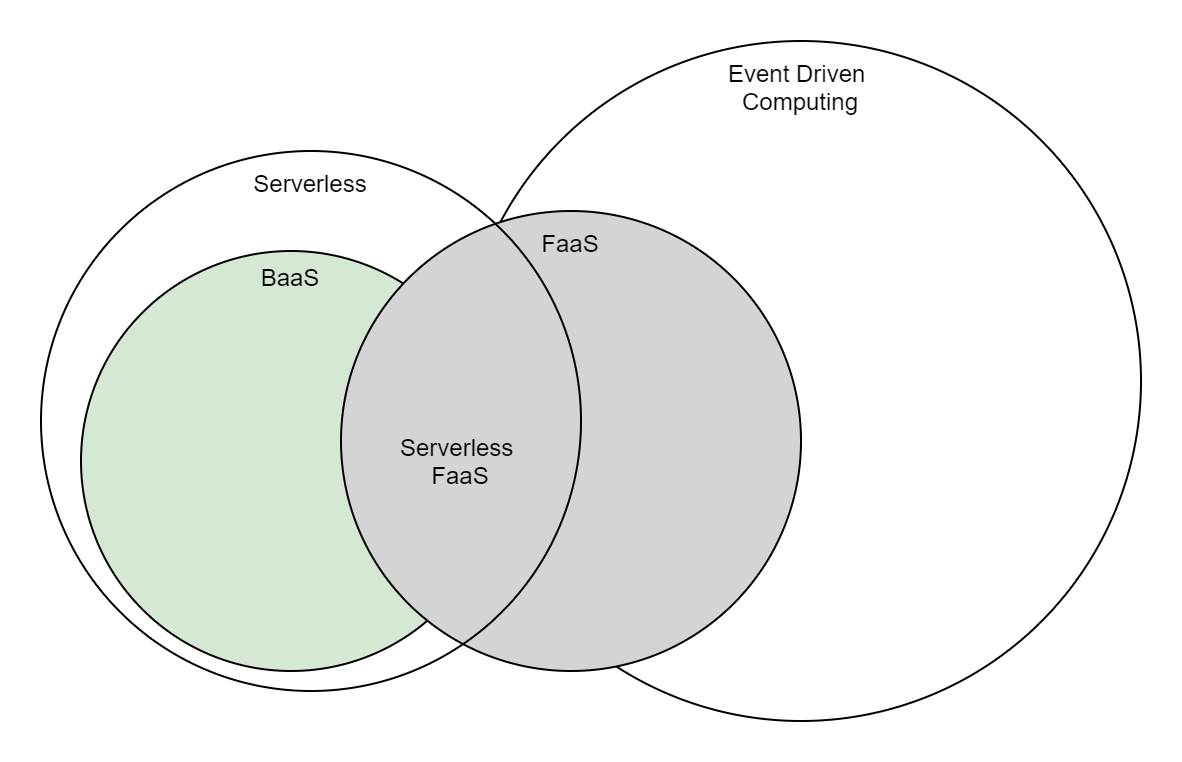
\includegraphics[width=0.7\textwidth]{Serverless}
\end{figure} 
Besteht eien Anwendung in der Folge lediglich aus den zwei \glqq serverlosen\grqq{} Komponenten, FaaS und BaaS, so ist häufig die Rede von einer \glqq pure serverless\grqq{}, also einer Anwendung, deren operationeller Teil vollständig an einen Cloud-Anbieter ausgelagert wurden und einer \glqq hybrid serverless\grqq{} Anwendung unterschieden \cite{leitner2019mixed}. Bei letzterem fungieren die Kunktionen häufig als sog. \glqq Glue\grqq{}, der meisten zeitlich variierend Aufgaben übernimmt, da IDLE-Zeit, wie man sie aus IaaS oder PaaS kennt, nicht berechnet wird.\\\\Nun mag der ein oder andere argumentiern, das ein Großteil der infrasturkurellen Aufgaben auch bei PaaS von dem Cloud-Anbieter übernommen werden, womit er natürlich recht hat. FaaS geht an dieser Stelle jedoch noch einen Schritt weiter. Bei Paas werden vorgefertigte \textit{Packages} einer Anwendung auf der Runtime der entsprechenden Plattfrom bereitgestellt, womit sich die Entwickler immer noch im die Anwenungsstruktur kümmern müssen \cite{kaplan2019framework}. In FaaS hingegen wird dieser Teil übernommen und der Entwickler konzetriert sich lediglich auf die Business logik und die jeweiligen Event-\textit{Trigger}.\\\\
Zuletzt soll noch auf einen weiteren Punkt, \glqq NoOps\grqq{}, eingegangen werden, der oft mit Serverless gleichgestellt wird. Es wird zwar durch die Übernahme des Loadbalancing, der automatischen Skalierung, Sicherheitsaspekten und Patches ein Großteil der Wartung ausgelagert, jedoch ist dies nicht mit der Annahme des Wegfalls der Operations von DevOps gleichzusetzten, wie suggeriert wird \cite{fowler2018serverless}. Es obliegt weiterhin den Entwicklern qualitativ hochwertigen Code zu schrieben und diesen in der Cloud-Umgebung zu testen, um dessen Performanz sicherzustellen. Die Komplexität entfällt daher nicht vollkommen, sondern verlagert sich zu einem gewiessen Teil \cite{eivy2017wary}. \textcolor{red}{Schaut man sich beispielsweise AWS an, so muss eine vielzahl an Konfigurationen vorgenommen werden. Zwar kann später eine vorhanden auf alle Funktionen angewendet werden, jedoch ist diese in der Folge von essentieller Bedeutung in einer riesigen \glqq Multitennacy\grqq{}-Umgebung.}\\\\% however, developers of serverless applications do not have to deal with any operational management with respect to provisioning, monitoring, maintenance,scalabilityandresilienceoftheserverstheapplicationisdeployedon \cite{baldini2017serverless}


\subsection{Potentiale und Herausforderungen}
Die im Folgenden aufgelisten Potential und Herausforderungen, denen sich Literatur und Anwender von FaaS gegenübersehen, sind zu Teilen dem Konzept selber, zu Teilen aber auch der Implementation der jeweiligen Anbeiter bzw. Open-Source Lösungen geschuldet. Es werden daher auf Seiten der Herausforderungen diese zunächst erläutert und falls in der Literatur bereits adressiert, vorgeschlagen Lösungen aufgezählt. Bei beiden, Potentiale und Herausforderungen, wird sowol Bezug auf FaaS als auch auf BaaS genommen, da diese beieden Kategorien in den meisten Fällen in Kombination genutzt werden bzw. architektionisch beding in Kombination genutz werden müssen [siehe Abbildung ~\ref{fig:serverlessBaaSandPaas} und \glqq statelessness\grqq{} Abschnitt \textit{Function as a Service}].\\\\\\
{\normalsize \textbf{Potentiale}}\\\\
\textbf{Kosteneffizienz}\\
\\\\
\textbf{Time to Market / Lead Time Development}\\
\\\\
\textbf{DevOps}\\
\\\\
\textbf{Testing}\\
\\\\
\textbf{Optimale Auslastung von Rechenzentren}
Greener Computing \cite{shafiei2020serverless} \cite{fowler2018serverless}
\\\\
{\normalsize \textbf{Herausforderungen}}\\\\
\textbf{Vendor Lock-In}
Auch wenn diese Eigenschaft sowohl 
\textbf{Physische Lokation}\\
Eine weiterer Punkt ist die physische Lokation der Funktionen. Dadurch, dass es dem Provider obliegt, die Ressourcen seiner Infrastruktur optimal zu nutzen, entscheidet dieser auch auf welcher Node eine Funktion ausgeführt wird. Platziert der Provider in der Folge Funktionen, die eine hohe Datenabhänigkeit haben, physische weit voneinander entfernt, so wird sich dies auf die Performance der Anwendung auswirken und letztlich als Latenz bei dem Endverbraucher zu spüren sein \cite{shafiei2020serverless}. Es gibt zwar bereits bei vielen Anbietern, wie AWS, Microsoft oder Google die Möglichkeit die Region beziehungsweise ein sog. Cluster festzulegen, jedoch lässt sich damit die Lokation lediglich eingrenzen, aber nicht rechenzentren-genau festlegen. Mit der Performance von \glqq serverful\grqq{}-Applikationen kann damit nicht gleichgezogen werden \cite{shafiei2020serverless}.\\\\
\glqq \textbf{Serverless}\grqq{}\\
Es ist an dieser Stelle zwar relativ trivial, trotz alledem ein Nachteil verglichen mit Lösungen wie PaaS oder IaaS. Die Rede ist von dem Verlust der serverseitigen Optimierung. Wie bereits durch den Namen deutlich gemacht, existieren die Server für den Nutzer nicht bzw. hat er bei einer auf BaaS basierenden Softwarelösung keine Kontrolle über das Backend. Er kann lediglich die Datenbanken, Objektspeicher oder Authentifizierung an die Struktur seiner Daten anpassen und über \glqq Regeln\grqq{}Zugriffsbeschränkugen umsetzen. Die Services sind von dem jeweiligen Vendor vorgegeben und können bspw. nicht nach dem \glqq Backend For Frontend\grqq{}-Muster\footnote{https://samnewman.io/patterns/architectural/bff/} auf die entprechenden Client-Typen, wie Tablet, Mobile-Phone oder Desktop angepasst werden. Es existieren von jeder Sorte (Datenbanken, Objektspeicher, Authentifizierung usw.) nur eine Version auf welche man beschränkt ist. Jegliche benutzerdefinierte Logik muss daher in den Client ausgelagert werden, da es nicht auf backendseitig implementiert werden kann \cite{fowler2018serverless}. Mit FaaS kann dieser Effekt gemindert werden, indem ein leichtgewichtige Logik in form von Funktionen serverseitig umgesetzt wird. Hierbei erfolg die Interaktion mit den unterschielichen BaaS-Servicen über die vom Anbieter beschränkten Trigger [siehe Abschnitt \textit{Function as a Service}].\\\\
\glqq \textbf{Statelessness}\grqq{}\\
Mit der \glqq statelessness\grqq{}, also der Zustandslosigkeit von Funktionen, geht eine weitere Problematik von FaaS einher. Der Kern von Anwendungen ist es Aufgaben zu lösen, wofür viele verschiedene Schritte von Nöten sind, welche sinnvoll miteinander verbunden werden müssen. So ist es auch bei dem funktionsbasierten Aufbau von Applikationen wichtig, dass diese untereinander kommunizieren können und den Programmstatus voneinander abfragen können, ohne das es zu Inkonsistenzen kommt. Bedingt durch die kurze Laufzeit der Funktionen ist es essentiell, dass auch der Austausch in entsprechender Geschwindigkeit erfolgt. Wie in einem Report von Berkeley \cite{jonas2019cloud} herausgearbeitet, erweist sich das schnelles und exaktes \glqq State-Sharing\grqq{} jedoch immer noch als problematisch dar, betrachtet man die Geschwindigkeit von \glqq Serverless\grqq{}-Anwendungen im Vergleich mit \glqq Serverful\grqq{}-Anwendungen.\\\\
Grund hierfür sind die von den Anbietern zur Verfügung gestellten BaaS-Lösungen für das persistente Speichern des Programmstatus. Objektspeicher der verschiedenen Anbieter (AWS S3, Google Cloud Storage, Azure Blob Storage) sind zwar nicht teuter sehr teuter wenn es um das Speichern mehrerer GB geht, jedoch sind die Kosten beim Zugreifen auf die Speicher hoch und die Latenzzeiten von bis zu 20ms zu hoch \cite{jonas2019cloud}. Die Key-Value-Speicher der Anbieter sind in diesem Falle die bessere Wahl, da ihre Ansprechzeiten mit 8 - 15ms geringer sind, jedoch sind sie, bezogen auf ihre Input/Output Operationen pro Sekunde, deutlich teurer als die der Objektspeicher.\\\\
Neben dem schnellen Informaitonsaustausch der Funktionen mit einem externen Speichermedium, kann es bei einer Kopplung von Funktionen aus performancetechnischen Gründen sinnvoller sein, den aktuellen Programmstatus direkt and die nächst Funktion weiter zu geben. Wie zuvor bei der \textit{physischen Lokation} der Funktionen erwähnt, ist es wahrscheinlich, dass Funktionen nicht auf der selben Node gestartet werden. Der Loadbalancer des jeweiligen Providers entscheidet je nach Auslastung der Infrasturktur, auf welcher Node eine Kopie der Funktion ausgeführt wird. Auch wenn im Idealfall die Weitergabe des \glqq application states\grqq{} schneller ist als der Zugriff auf ein externes Speichermedium, so wird dies durch \glqq Startup-Latencies\grqq{}und physischer Distanz wieder relativiert. Um dem entgegenzuwirken schlagen Shafiei et al. \cite{shafiei2020serverless} vor, mit einem \textit{Dependency-Graphen} miteinander verwobene Funktionen zu kennzeichnen und direkt bei dem initialen Aufruf einer Funktion mögliche Folgefunktionen zu starten.\\\\
Würde man dem Nutzer die Möglichkeit geben zu bestimmen auf welcher Instanz (Node) eine Funktion laufen soll, so das Konzept von FaaS damit untergraben werden (siehe \textit{Optimale Auslastung}). Es würde dazu führen, dass erneut Kapazität zurückgehalten wird, über welche der Provider nicht mehr frei verfügen könnte. 
\begin{figure}[H]
\caption{Dependency Graph nach \cite{shafiei2020serverless}}
\label{fig:dependencyGraph}
\centering
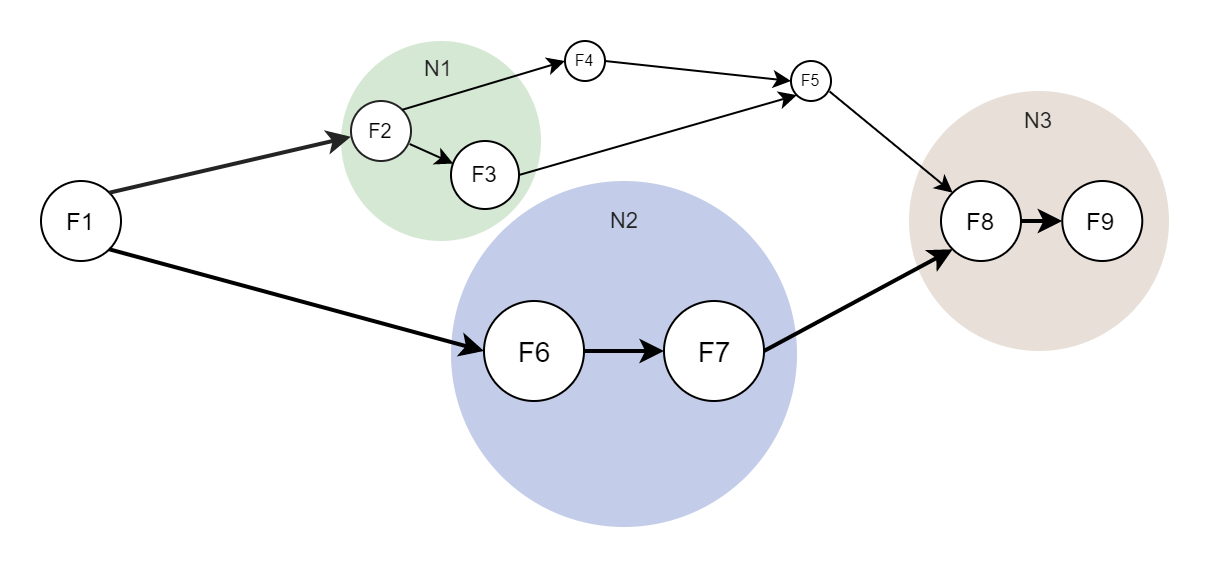
\includegraphics[width=1\textwidth]{DependencyGraph}
\end{figure} 
Wenn jeder Nuter bestimmen könnten auf welcher Node, bspw. Node-X, seine Funktionen laufen sollen, um den Progrmamstatus mit so wenig physisch bedingter Latenz wie möglich weiterzugeben, so wäre eine optimale Auslastung nicht mehr garantiert. Der Provider müsste stets Kapazität von Node-X zurückhalten und könnte sie nicht für andere Nutzerfunkitonen freigeben. Er muss stets einen Teil der Kapazität von Node-X zurückhalten, für den fall dass inaktive, aber der Node zugeteilte Funktionen aufgerufen werden. Mit einem \textit{Dependency-Graphen} wie in Abbildung ~\ref{fig:dependencyGraph} zu sehen würde dieses Problem umgangen werden. Der \textit{Load-Balancer} des Anbieters könnte unbeinträchtigt die Funktionen wie gewohnt je nach Auslastung auf freie Nodes verteilen, da er die korrelierenden Funktionen \glqq gleichzeitig\grqq{} starten kann. Da die Latenzen beim Starten eines Services erheblich höher sind, wobei die Programmiersprache dies zusätzlich beinflussen kann \cite{manner2018cold}, als jene durch die Lokation bedingt \cite{aditya2019will} \cite{jackson2018investigation}, würde deren Eliminierung die Weitergabe des \textit{States} erheblich beschleunigen.\\\\
Generell betrachtet könnte die Geschwindigkeit der Kommunikation von Funktionen untereinander beschleunigt werden. Verbindet man das ganze noch mit einem einfachen neuronalen Netz, um beispielsweise vorherzusagen mit welcher Wahrscheinlichkeit Funktion zwei (F2) im Vergleich zu Funktion sechs (F6) angesprochen wird, so könnte die Performance sogar noch ressourcenschonender auf Seiten des Cloud-Providers gestaltet werden. Zunächst käme es entweder zu einer höhreren Belastung, sollte man zu Beginne alle Funktionen starten oder zu einer höheren Latenz, sollte man die Funktionen einzeln starten und aus dem sich ergebenden Verlauf lernen. Nach einer kurzen Lernphase würde die Auslastung der Infrastruktur jedoch erhöht werden.\\\\
\glqq \textbf{Multitenancy}\grqq{}\\
Obgleich das Konzept von FaaS darauf beruht, dass der Anbieter eine Vielzahl von Funktionen verschiedener Kunden steuert und pflegt, so soll sich jeder Kunde fühlen, als sei der der Einzige. Allerdings stellt dies die Betreiber der Plattformen vor weitere Herausforderungen, da sie die Ressourcenisolation sowie Zugriffsbeschränkugen zuverlässig gewährleisten müssen. Dies ist jedoch leichter gesagt als getan, da es teilweise nicht nur von dem Provider selber, sondern auch von der richtigen Konfiguration der Sicherheitseinstellungen der Nutzer\footnote{https://awsinsider.net/articles/2017/06/20/voter-data-leak.aspx},\footnote{https://searchsecurity.techtarget.com/news/450422962/Another-AWS-cloud-data-leakage-due-to-misconfiguration} abhängt, ob die Daten unzugänglich für Dritte sind.\\\\
Obwohl Anbieter wie AWS Mittlerweile erfahren genug sein sollten, dass solche Probleme nicht mehr zu erwarten sind \cite{fowler2018serverless}, ist weiterhin Vorsicht geboten. Es nichts an der Tatsache, dass auch sie sich mit Sicherheitsaspekten, der Robustheit und Performance ihrer Infrastruktur ständig weiter auseinadner setzten müssen. Kein Kunde darf die Daten eines anderen sehen, kein Fehler die Stabilität anderer Funktionen gefährden und kein plötzlich auftretender \textit{Spike} eines Kunden die Performance der Funktionen eines anderen beeinträchtigen. Das Zusammenspiel von RPCs und der Containersicherheit muss dauerhaft gegeben sein und durch sorgfältiges \textit{Security Managament} sichergestellt werden \cite{mcgrath2017serverless}. \\\\
\textbf{Testing}\\
\\\\
\textbf{Cold-Starts}\\
\textit{Cold Starts} beziehen sich auf das Starten eines Containers, in welchem eine Kopie der benötigten Funktionen zur Verfügung gestellt wird. Ist eine Funktion lange nicht genutzt worden oder wird zum ersten Mal angesprochen, so muss für die Ausführung zunächst alles vorberietet werden. Vor allem bei sehr kurzen Funktionen stellen sie ein erhebliches Problem dar, da ihre \textit{Start-Up}-Zeit bis zu ein Zehnfaches der eigentlichen Ausführungszeit einnehmen kann \cite{shahrad2019architectural}. Ein Container muss auf einer Node gestartet werden und die Funktion, sowie deren Abhänigkeiten geladen werden. Die Zeit die es dauert, bis die Instanz bereit ist hängt dabei von verscheidenen Faktoren, wie der Programmiersprache, der benötigten Bibliotheken (\textit{Libraries}), der Größe der Funktion (menge an Code) und der Hardware \cite{shafiei2020serverless} \cite{jonas2019cloud} ab, auf der die Funktion instantiiert wird. Wird eine Funktion dabei sehr frequentiert aufgerufen, so halten die Plattformen diese Funktionen für eine gewisse Zeit vor (\glqq warm\grqq{}, bei AWS bis zu einer Stunde \cite{roberts2017serverless}, wodurch die Wahrscheinlichkeit eines erneuten \textit{Cold Starts} gegen Null tendiert. Bei Funktionen die hingegen nur einmal pro Stunde bemüht werden, sind die Folgen von \textit{Cold Start} deutlich häufiger zu spüren \cite{roberts2017serverless}.\\\\ Um dem entgegenzuwirken schlägt \cite{castro2019server} vor, eine Art stammzellen Container vorzuhalten. Diese würden für die unterstützten Programmiersprachen bereits instantiiert aber leere Container vorhalten. Diese Container sind nicht Kundenspezifischen und generisch nutzbar. Damit würden zwei der obene genannten Punkte, die Programmiersprache und die Hardware, welche die \textit{Startup}-Zeit der Funktionen negativ beeinflussen, eleminiert werden. Lediglich die größe der Funktionen und deren \textit{Dependencies} müssen noch geladen werden. \cite{ishakian2018serving} hat zudem gezeigt, dass mit der Erhöhung der Speicherkapazität die Zeit bis eine Funktion bereit ist einen \textit{Request} zu bearbeiten verringert werden kann. Kombiniert man dies mit dem Stammzellen-Ansatz, so wird das Laden des Programmcodes und der \textit{Libraries} beschleunigt. Natürlich kommt der zusätzliche Speicher nicht umsonst, jedoch liegt es in dem Fall bei dem Unternehemn zwischen den Mehrkosten und dem Performancezuwachs abzuwägen. \\
%Keep alive \cite{lloyd2018improving}
\newpage














\section{Guidline on Migration}
The below-presented guideline for migrating parts of existing microservice architecture to the relatively new cloud-computing concept, Function as a Service, is structured as follows. At first, the decision to migrate is questioned by challenging the motives of adopting this new technology and giving advice on when to migrate. Afterwards, criteria for selecting the right service will be stated, which gear towards the possibilities that come along with FaaS. When a reasonable service has been found, a provider needs to be identified, which best meets the company's requirements. There are two types of providers that primarily differ in the service-ecosystem inherent to them and the degree of vendor lock-in. Whereas proprietary platforms like AWS, Azure, or Google provide a vast ecosystem of feature services and backend as a service offering, open-source frameworks like OpenWhisk, Fission, or Kubeless dedicate greater control to the developers. When implementing FaaS, the open-source solution can be far more adjusted and configured to best suit an organization's needs. Next, impacts on the general process of software development, the \glqq Dev\grqq{}-part in \textit{DevOps}, will be investigated. Changes in organizational structures regarding the development team, as well as effects on the CI/CD pipeline, challenges faced with local testing, and the VCS, will be addressed. With the development process covered, the guideline on migration will end with the operational part, which will be taken into account. Alternations on the process of monitoring, maintenance, and testing instances will be covered, and advice on coping with them will be given.\\\\ To better follow along with the guideline, the subsequent section will provide an overview of the current microservice infrastructure. The development process, as well as the operational tasks, will be described, along with the underlying service-landscape.


\subsection{Describing the existing architecture}
In the afterwards, the current process of development and operations is described, to later on better illustrate the effects of introducing Function as a Service to the existing microservice architecture [see \cite{newman2015building}]. Figure ~\ref{fig:devops} provides a high-level overview of the prevalent DevOps Pipeline. In the final stage of this section, by summing up on the construction of the guideline, figure ~\ref{fig:devops} will be examined regarding necessary changes. \\\\
Starting with the development team, it consists of around eleven developers that are working after Scrum the agile process framework [see \cite{pichler2013scrum}]. During a sprint, the team splits up in groups of two to four, to work on the tasks they commited on. Therby the main language used for developing the services is Java. Following a common pattern, the basic structure of a service is defined in a YAML-file, configuring its endpoints, parameter types for request and responses, descriptions and other paramerter. The YAML will be passed to swagger-codgen which will generate the basic servie structure. Using Maven. an automation tool for service developemnt, the servie can be built for the first time, getting ist dependencies form the service POM. In the POM, which basically is a xml file including information about the service. The fiel documents target locations, dependencies, verison and other defualt configurations for building the service. With the service being built, the business logic can be implemnted. To keep track of differnet versions of services and entire service landscape of the platform, a VCS like Github, Bitbucket or Tortoise can be used. From time to time, while working on the business logic, the service will be built and the tested. The test are executed in the local developemnt environment, using mock data form test-databases. By time the service is documented, a PR can be created. To gauartee a certain service quality, to be more precise code quality, all services emabrace parts of a so-called core service. The core-service  enfroces certain standard functionalities in terms of logging,   
\begin{figure}[H]
\caption{DevOps Pipeline}
\label{fig:devops}
\centering
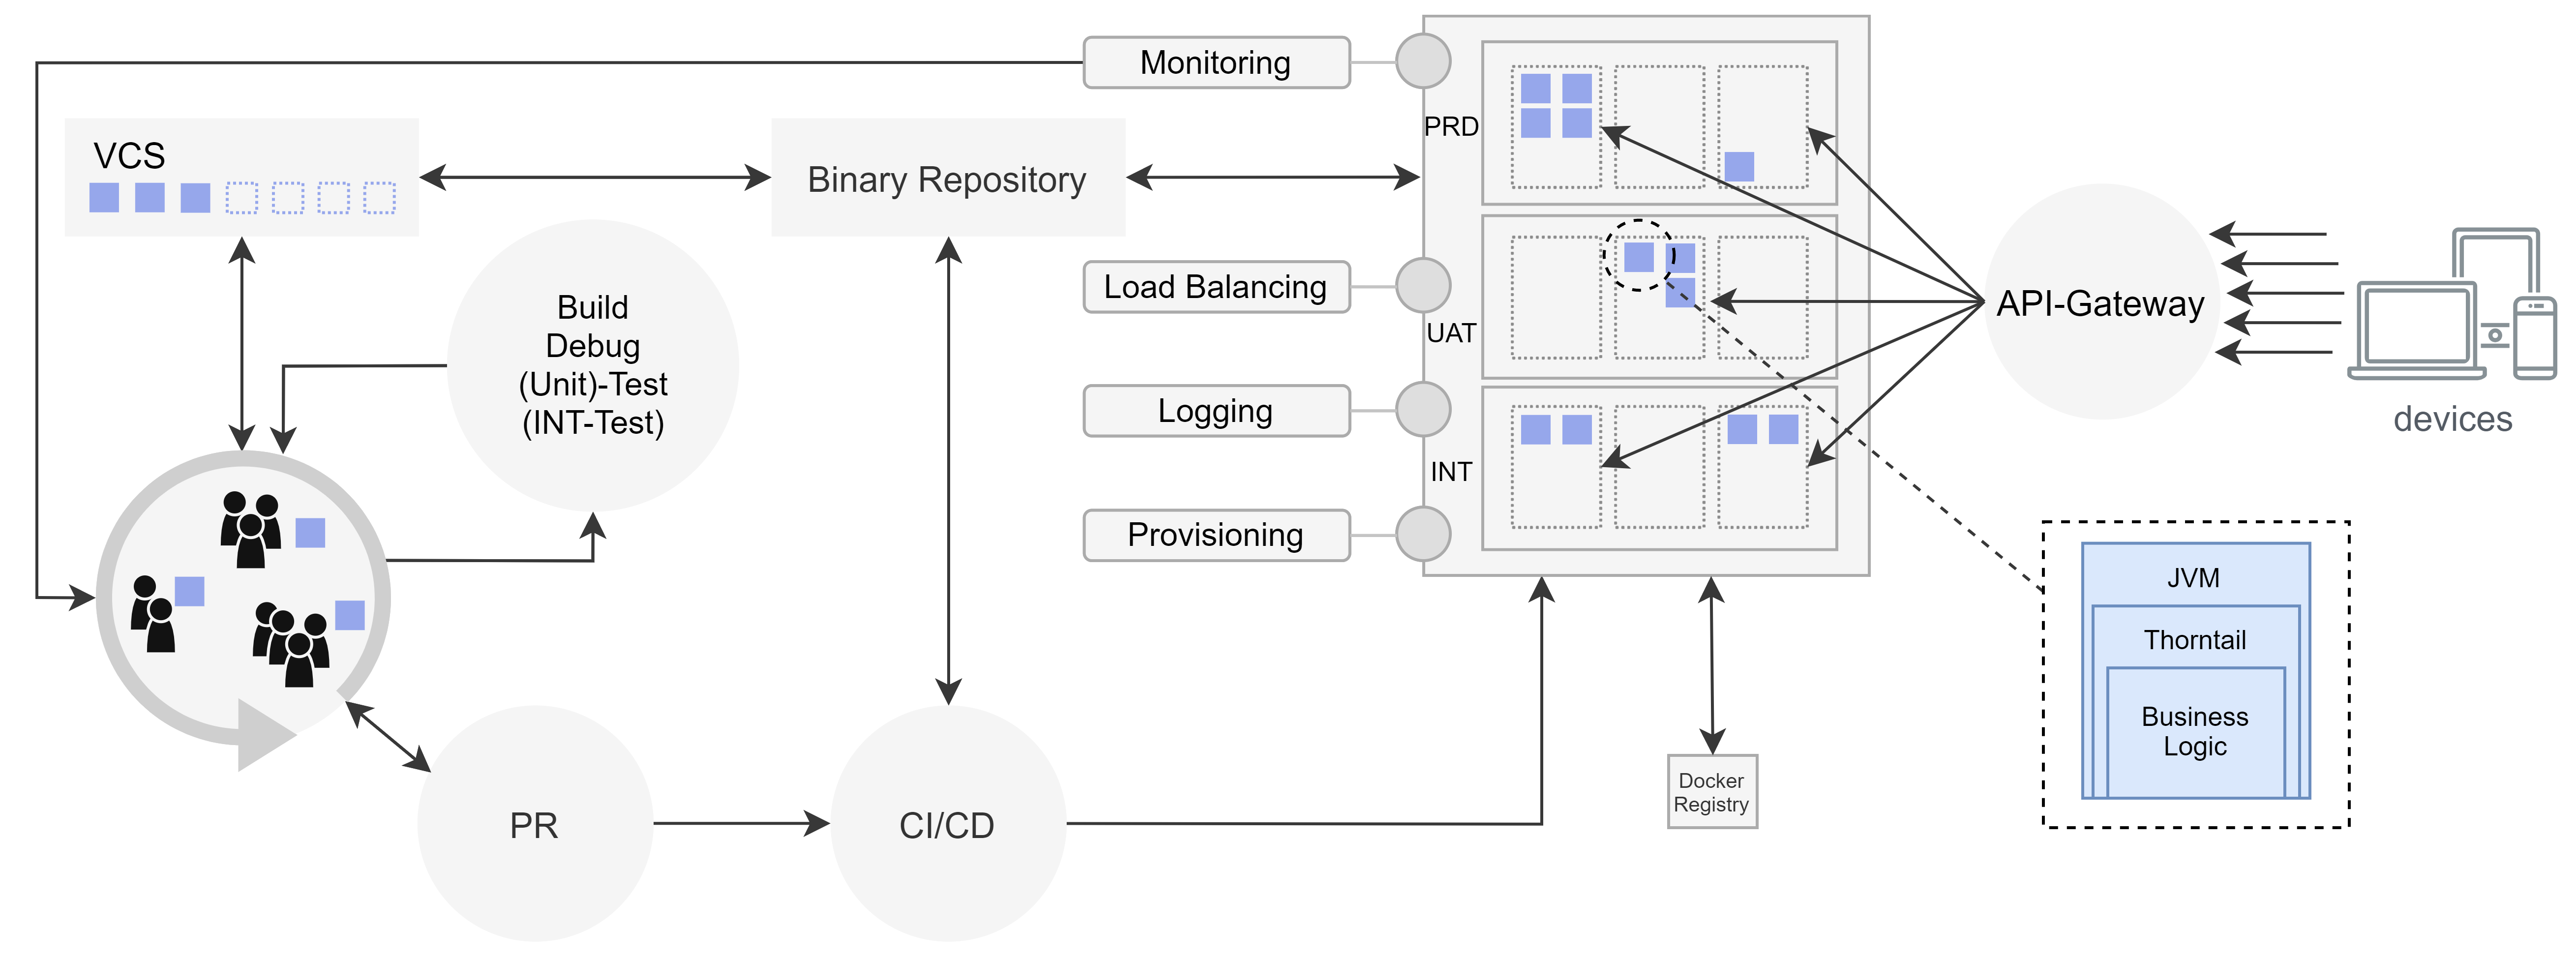
\includegraphics[width=1\textwidth]{DevOps}
\end{figure}
For the CI/CD pipeline different procducts can be used for automaton. Two popular choices are Jenkins and TeamCity. The puropse of the pipeline is to build the service, execute tests, and provides the servies war-files and jar-files to the Binary Repository. The Binary Repository istsle is connected with the VCS as well as with the CI/CD pipeline. By triggering a build process for one of the services its binarys will be pushed to he server platforms.

Binaries into docker contianer as well as git, JVM etc. all then stored as a docher image, which later on has all the information so jenkins only has to trigger the build of a specific image. Therby the process can be speed up due to not having to build run or test anyting. When a new instance of a service is needed, it can be loaded directly from the image repository. To ease working with containers, kubernetes can be installed. Kubernetes which is an open-source framwork for automating deployments, scaling and management of containerized applications. 


\subsection{Scrutinising the Decision of Migration}
Whereas migrating from a monolithic application to serverless, respectively, Function as a Service, seems far more challenging, due to the assumed size and complexity of the application, migrating from a microservice-architecture can be challenging as well. With a monolithic application, functionalities need to be identified in the first place and afterwards be broken down into many small functional sections. Microservices, on the other hand, might already be small enough that they supply only certain functionalities. Still, in some cases, they do incorporate too many functionalities to be converted to functions right away. Nevertheless, dealing with the issue of outsourcing the currently inherent state of services, as well as reducing dependencies and optimizing code remains.\\\\ Before starting to introduce this new technology into the service landscape, it is essential to contrast the current state of the system with the desired state of the system. When a system is already composed of many small services, the underlying infrastructure likely consists of VMs or containers. Those containers often run in a PaaS environment, and it is not possible to scale them to zero to free reserved computing capacity in favor of other services to consume it. To do so or even to outsource the expense of provisioning services, managing the underlying infrastructure and coping with operational tasks, such as monitoring, load balancing, etc., function as a Service can help to achieve this desired state. The restrictions that come along with the ease of development have to be traded off against its benefits.\\\\ To profit as much as possible of introducing FaaS, the services, which should be migrated, have to be inspected regarding dependencies, size, version, language, and complexity. It is recommended to reduce dependencies them to a minimum, due to their effect on the star-up time of the container the function runs in \cite{manner2018cold}. Especially with Python, Nodejs, and Java \cite{puripunpinyo2017effect}, loading all dependencies required, which might again interconnect with other dependencies, the number of dependencies will have an impact on cold starts. The next issue which needs to be addressed is state management.\\\\ As mentioned in section two, \textit{benefits and drawbacks}, there is no persistent state an application can rely on. There actually is a persistent state in the container of a function, but whether an incoming request will hit a particular container, is unpredictable. When a service does not receive any request or is running for a long time, the provider will eventually kill its container to free capacity. In the case of AWS Lambda, the current maximum amount of time, of a frequently called function until it gets killed, is 45 minutes\footnote{https://aws.amazon.com/de/lambda/}. Later on, when comparing cloud providers with open-source frameworks, there will be guidance on fining an appropriate solution to meet a company's purpose. Still, for now, the following must be considered. When using an open-source framework like OpenWhisk, the external state management system can be covered with Redis or another low latency database. Whereas using a cloud provider platform, one of its integrated database solutions will presumably be the best choice. If it is necessary to have full control over the performance and configuration of the database, an open-source framework has to be chosen.\\\\ The latency and frequency of a service will also decide upon its aptitude for being a candidate to get migrated to FaaS. If the service is called very frequent and experiences most of the time very high traffic, the concept of function as a Service will not apply to it \cite{jonas2019cloud}. Due to a limit of concurrent running functions, that can vary between the different providers and frameworks; incoming traffic can only be handled upon a certain amount. Moreover, the same application experiencing the same amount of traffic, once running on a FaaS platform and once running in a docker container in a PaaS environment, will be more expensive implemented with FaaS, than it will be with PaaS \cite{jonas2019cloud}. Therefore, services with various workloads, having eventually high peeks and then some time of inactivity, are more applicable to the concept of serverless, than their counterparts.\\\\ Latency should also not be a critical component due to the before mentioned cold starts. Latency sensitive applications like trading platforms, which strongly rely on real-time data, are not a suitable candidate for Function as a Service. Another pitfall is the promise of not having to maintain, provision, scale, or monitor the infrastructure and thereby reducing complexity and operational tasks. On one side, the cloud provider will, to some extent, take care of load balancing, scaling functions up and down, and providing monitoring solutions. On the other side, new complexity will appear in other areas. The issue of mono-repo and poly-repo arises, as discussed in a later section, followed by the necessity to learn the provider's DSL. Furthermore, the team needs to acquire skills to configure security policies correctly, interconnect function with each other, define different triggers on functions, deal with concurrency setting \footnote{https://docs.aws.amazon.com/lambda/latest/dg/configuration-concurrency.html}, and many more aspects add complexity to new fields. If the company aims at reducing infrastructural complexities, then Function as a Service can support at the listed tasks, but when its primary purpose is to reduce operational efforts, as often suggested with the term \glqq NoOps\grqq{} \cite{eivy2017wary}, FaaS, again, is not the right choice.\\\\ Lastly, attention needs to be drawn to the programming language and lead time development. FaaS can provide a reduction in lead time development and time to market, thanks to its small codebase and rapid development [\cite{sewak2018winning}, \cite{leitner2019mixed}]. Developers can make changes, fix issues, test, and finally deploy a new version to production in a view minutes. Prerequisite, even though this might sound trivial, is the platform language support for the language used in the application or service. Although the big cloud providers already support many programming languages, application logic might have to be rewritten, if that specific language is not supported. In the case of version incompatibility, the application needs to be rewritten as well. Especially when the provider's version is below the version of the application, it becomes an issue.


\subsection{Balancing between Open-Source and Cloud-Vendor}
Choosing an open-source over a cloud vendor, or the other way round, depends on the purpose of utilization. Neither is the so-called vendor lock-in a drawback nor a limitation, compared to an open-source solution; it is solely a tradeoff between the benefits of two different approaches of the same model. Nevertheless, the decision on one of them will affect the possibilities in the process of development and migration. To answer the question on which one to choose, the following things need to be considered.\\\\If the primary purpose is to start rapid development with not having to configure any infrastructure, a cloud vendor seems to be a promising solution, especially when a project has no legacy application that needs to be refactored or rewritten. Which of the vendors exactly is to be taken, is dealt with in the following section.\\\\With Amazon Web Services (AWS) Lambda, Microsofts Azure Functions, IBM Cloud Functions or Google Cloud Functions, each of the large serverless providers has a considerable amount of services in its ecosystem. Moreover, the ecosystem is utterly compatible with itself, making the need to find a custom workaround for processes like CI/CD obsolete. AWS and Azure even provide a premade solution for that purpose. E.g. an application requires user authentication, different types of databases, messaging services and hosting, each of the platforms mentioned above can satisfy these needs. Adding to that, they provide an appealing pricing model with free contingents each month, which makes them a feasible candidate for experimenting with different cloud service \\\\Unfortunately, these benefits do not come without restrictions. By ceding the responsibility of provisioning, load-balancing, scaling, error-handling, monitoring and many more duties to the cloud provider, one is dependent on the tooling provided by the platform. Just because the responsibility of maintenance and provisioning is outsourced to the provider, this does not mean that there is no need for an additional monitoring practice, as later stated in \textit{implications on monitoring}. In case something goes wrong on the platform, it is recommended to have, besides the tools offered by the provider, additional information to reproduce the error, find its cause and solve the problem. Another point that has to be considered is the outage of the platform, which is per se not exclusively a cloud provider issue but something that might be dealt with. A possible solution to this is a framework sitting between development and the platform, enabling multi-cloud application that can produce relief.\\\\ Depending on how one looks at it, the services can be depicted as an advantage or disadvantage. Even though the different services undertake many tasks, for many tasks, additional services need to be consulted. In the case of AWS, the platform do scales, monitors and sends messages, but the services needed to do so are more than a view.\\\\If the concept of FaaS should be introduced to a company or project along with staying in control of the entire infrastructure, a cloud provider solution is not applicable. In this case, one of the large numbers of open source providers needs to be chosen. If the present application is built upon Kubernetes, for the purpose of virtualization, Kubeless, OpenWhisk and Fission are feasible FaaS options, that can be integrated with little effort \cite{palade2019evaluation}. Using an open-source provider, configurations in terms of computing time and resource capacity can be customized, due to being in control of the platform. Introducing FaaS to an upfront ecosystem will increase its performance and efficiency by freeing unused resources. At the same time, and operations teams will be needed that is in charge of implementing a monitoring solution and configuring the properties of the system \cite{mohanty2018evaluation}.\\\\ 


\subsubsection{Vendor analyses}
Depending on the decision made in the previous section, there are various frameworks and platforms at choice. Below, three solutions for each approach are presented. Starting with open-source frameworks, Fission, Kubeless, OpenFaaS and OpenWhisk will briefly be introduced in the following.\\\\ \textit{Kubeless} is a Kubernetes native serverless framework, being a straight forward extension for a Kubernetes API-Server. Kubeless itself has no API-Server and no data store to store objects since it is reusing everything from Kubernetes. For scaling, Kubeless makes use of the Horizontal-Pod-Autoscaler, for monitoring Prometheus is used and for deployment via the API, ConfigMaps and Ingress are utilised\footnote{https://kubeless.io/}. Thus being built on top of Kubernetes, making use of its CRDs\footnote{https://kubernetes.io/docs/concepts/extend-kubernetes/api-extension/custom-resources/} to create functions, users familiar with the Kubernetes-API can process as usual. The language-runtime itself is encapsulated in a container image which will be set in the Kubeless configuration. A list of supported runtime can be found on github\footnote{https://github.com/kubeless/runtimes/tree/master/stable}. Each function will be deployed in a separate Pod, supervised by Kubernetes HPA. When a function is not used, the HPA will kill the pod to free capacity. Prerequisite is the deployment of the function with a CPU request limit. Depending on the runtime, metric data can be monitored by Prometheus.\\\\ \textit{Fission} is a serverless framework build on top of an underlying Kubernetes infrastructure. Just like Kubeless, Fission does not inherit a resource store and therefor depends on communicating with the Kubernetes API service\footnote{https://docs.fission.io/docs/concepts/components/core/controller/}, in order to get access to secrets and \glqq ConfigMaps\grqq{}. Supporting a large number of programming languages\footnote{https://docs.fission.io/docs/languages/}, with Fission, CPU and memory resource limits can be configured. Two aspects which make Fission unique compared to the other three is, for one thing, its ability to define the number of pre-warmed pods and for another thing its richness of possessing a Workflow-System. Whereas the pool of pre-warmed pods can be utilized to mitigate the cold start issue, the Workflow-System makes it easier to handle an increase in functions and execute more complex workflows [see \cite{kritikos2018review}]. In contrast, Kubeless uses event chaining to create workflows which makes it harder to maintain the workflow graph.\\\\ OpenFaaS\footnote{https://www.openfaas.com/} provides a so-called \textit{faas-provider} interface, letting it integrate with any provider that has implemented the interface. Currently, these providers are Kubernetes, Docker Swarm and \textit{faas-memory}\footnote{https://docs.openfaas.com/architecture/faas-provider/}. Each function will be packaged into a docker image and deployed via the OpenFaaS CLI. With its API-Gateway, OpenFaaS can respond to any event, and by making use of its auto-scaling functionality the min/max amount of replicas can be configured\footnote{https://docs.openfaas.com/architecture/autoscaling/}.\\\\ Lastly, OpenWhisk is a serverless framework which has initially been developed by IBM and is now backed by Apache. Because OpenWhisk was backed by a large company, its application model is often referenced in literature when the application model of other large cloud providers is indicated. it can be assumed that other vendors are using a similar concept due to OpenWhisk being provided in a large cloud environment \cite{van2019spec}. As an orchestration tool, Kubernetes can be used in conjunction with OpenWhisk, as well as IBMs Composer. As with the other three language runtime support here too, is quite large, ranging from Go over Java and Python all the way to Nodejs\footnote{https://openwhisk.apache.org/}.\\\\ In addition, four open-source frameworks support three different types of triggers [see figure ~\ref{fig:openWhiskProgrammingModel}], namely HTTP, Event and Schedule, natively. Moreover Fission, Kubeless and OpenFaaS are written in Go, OpenWhisk in Scala.\\\\ Concurrency test on Kubless, OpenFaaS and Fission have shown that the latter framework with 2ms has the fastest response time of all three. Moreover, its response times are consistent regardless of the number of replicas present and the number of concurrent users \cite{mohanty2018evaluation}. The test was conducted with 1, 25 and 50 replicas. Kubeless and OpenFaaS experience an exponential increase in response-time, with OpenFaaS showing a decrease in response time the more replicas are prevalent.Finally, Fission has a success ratio of 100\% in all three tests, whereas Kubeless and OpenFaaS are facing a slight decrease from one to four percent.\\\\ Speaking of proprietary Function as a Service solution, the three market leaders are AWS, Azure and Google, respectively \cite{kumar2019serverless}. By offering a vast amount of tooling and services, it can be challenging to choose one of these three, even though their underlying model does not differ a lot. With all three providers, functions are billed on their number of incoming requests, the time a function runs to process a request, billed at a tenth of a second, and the memory allocated to a function. Due to the cloud, especially serverless, being such a volatile market, listing on pricing and memory size would presumably be obsolete in a few months, referencing to the provider's platforms. Instead, performance evaluations, concurrency and runtime will be used as an indicator for choosing a platform.\\\\ Currently, on AWS, the maximum amount of time a single function will last is 15 minutes. After that time, the container the function is running in will be killed, no matter whether it has finished processing. On Azure functions, by default 5 min are the maximum, which can be upgraded to 10 if needed. Google Cloud Functions comes last, with a standard execution time of one minute, which can be raised up to 9 minutes. Looking at the limits on concurrent instances, on AWS Lambda, the limit varies between 500 - 1000 depending on the region, although the burst concurrency limit can reach a maximum of 1000-3000 concurrent instances. This those numbers only describe the initial limits, allowing to add each minute 500 additional instances. At this point, it is important to mention that these limits refer to an account, not a function. 1000 might sound a lot in this context, but depending on the number of functions, 1000 concurrent running functions can be reached quite fast.\\\\ Regarding the execution time of AWS Lambda and Azure Functions, the platforms not only differ in the execution time of cold and warm starts but also when comparing two programming languages. As a compiler language, with its JVM, Java functions require more time to execute than an interpreted language like JavaScript. Test have revealed, that there can be a significant gap receiving a result with a difference from 0.6 (JavaScript) and 1.7 (Java) seconds from cold to warm start on AWS and 9.8 (JavaScript) and 24.8 (Java) seconds on Azure \cite{manner2018cold}. Moreover, Manner et al. have detected that the cold start time of Java compared to JavaScript is on each memory size on AWS by a factor of two to three higher. Azure with a factor of 2.5 shows equal latencies in cold starts. Due to different memory allocation approaches, explicit configuration on AWS and dynamic allocation on Azure, the findings of latencies between the platform can not be compared to each other directly \cite{manner2018cold}.\\\\ Observed by other researchers as well, AWS appears to be very predictable in its memory size performance ratio \cite{pawlik2019performance}. Even though the performance memory ratio is stable, the maximum CPU-performance increase seems to reached with 2048MB memory. 3008MB exhibits no significant improvement. IBM and Google experience similar ratios. In terms of delay, it viewer the larger the memory size is, whereas Googles start delay are generally constant. On IBM tough, it seems that resource-consuming increases when a larger amount of resources is requested. \cite{pawlik2019performance}. Function throughput, which is an indicator of concurrent processing, AWS reaches its maximum throughput most rapid, followed by IBM, Azure and Google, respectively. Whereas Google at the lower end increases throughput steadily, with a rise in calls, AWS stays sturdy at its maximum. IBM and Azure experience a small decrease over a long time. Lastly looking at the runtime overhead of AWS, IBM, Google and Azure, on AWS it is almost evenly low regardless of a compiler or interpreter language. On Azure, C\# creates the least overhead, still being twice as much as AWS highest language runtime overhead, and Python the largest. On IBM the overhead is similarly high across the languages, and Google has the least overhead with Nodejs \cite{pawlik2019performance}.\\\\ Another point to consider, when migrating parts of existing architecture, in this case, a microservice architecture, to Function as a Service is orchestration. The orchestration solutions vary between different cloud and open-source providers. Thereby the respective orchestration tool decides upon performance when executing functions in parallel and upon runtime overheads. Moreover, pricing needs to be considered when configuring concurrency options across different providers. As mentioned before, depending on the memory size chosen, the performance can be increased, but pricing will increase as well. Whereas in small projects, concurrency and pricing might not be the current issue, in medium to large-sized projects, memory and pricing of the various providers should be taken into account.\\\\ As stated in section ... \textit{Benefits and Drawbacks} under \textit{statelessness} when chaining functions, passing state from the sending to the receiving function is key for intercommunication. With a higher speed of state-transfer, latencies are reduced. Only with a seamless interaction of functions complex applications can be built on a larger scale. Looking at proprietary cloud providers, the two largest platforms, AWS Lambda and Azure Functions,  will be depicted and further investigated. On the side of open-source frameworks, OpenWhisk is taken into consideration.\\\\ Lopes et al. have investigated on the named frameworks in greater detail and detected significant differences on state transfer both sequential and parallel orchestration \cite{lopez2018comparison}. For the tests conducted, all functions were executed on warm instances/ containers, to mitigate inaccuracies caused by varying cold-start times [see \cite{manner2018cold} and \cite{jackson2018investigation}]. In terms of executing sequential functions, called sequential processing, IBM's Composer and ASF proved to be significantly faster compared to ADF. The overhead, describing the time that was not used to carry out any processing of business logic inside a function, was 1.1s for IBM Composer and 1.2s for AWS Step Functions with 40 functions connected in series. Azure Durable Functions, on the other hand, took 8s for the same 40 functions. In further implementations with [5, 10, 20, 40 and 80] it turned out, that IBM Composer only supports the orchestration of functions up to a number of 50 sequential functions. Anything beyond that limit has to be controlled by a third party orchestration tool \cite{lopez2018comparison}. ADF and ASF, on the other hand, can define workflows which can run for days and months.\\\\ The evaluation of the overhead for functions connected in parallel was carried out for ASF and ADF, solely. Starting with five functions and, as described above, scaling up to 80, the results showed a significant increase in overhead of Azure Functions. With a total of 80 functions, Azure Durable Functions with an average overhead of 32.1s had almost twice the volume of AWS Step Functions with an average overhead of 18.3s. The results also suggested that ASF is more reliable than ADF in predicting the overhead to be expected. Microsoft's overhead has not always grown exponentially like Amazon's, making it difficult to predict future behaviour.\\\\ When evaluating the suitability of parallel function execution, IBM's Composer dropped out of the test portfolio right from the start, since parallel function execution was not supported [as of 2018 \cite{lopez2018comparison}]. Meanwhile [stand 2020], IBM includes support for parallel execution of functions via Composer. Furthermore, IBM states that parallel execution is not restricted to a certain number of concurrent functions and can be configured as needed \footnote{https://github.com/apache/openwhisk-composer }. However, it is explicitly mentioned that the Composer theoretically has no limits, but OpenWhisk does. Exceeding Openwhisk's limits of parallel execution will result in failures: \glqq[...] many concurrent invocations may hit OpenWhisk limits leading to failures: failure to execute a branch of a parallel composition or failure to complete the parallel composition [...]\grqq{} \footnote{https://github.com/apache/openwhisk-composer}. The current limitation of concurrent functions in OpenWhisk is placed at 100 functions per namespace.\\\\ Finally, the three orchestration solutions were examined concerning transferring application state. Due to the state limitation of ASF to 32KB that can be passed to the next function, the same size was chosen for the other two solutions as well. This time only five sequential functions were tested. In 2018 the official limit of IBM Cloud Functions was at 1MB, being raised upon 5MB by the time writing this thesis \footnote{https://cloud.ibm.com/docs/openwhisk?topic=cloud-functions-limits}. ADF enables state transfer up to 60KB. It was found that IBM Composer and AWS Step Functions had an overhead of 175.7ms and 168.0ms, respectively,  when executed without any additional payload. With payload, the overhead in ms for Composer was 298.4ms and 287.0ms for AWS Step Function, which represents an increase of 70\% [see figure ~\ref{fig: orchestration}]. Azure Durable Functions stood out clearly in this test. With an overhead of 766.2ms without payload and 859.5ms with payload, the basic overhead is significantly higher than with the previous two but only increases by 12\% under load \cite{lopez2018comparison}.
\begin{figure}[H]
\caption{Overhead bei 5 sequentiellen Funktionen mit einem Payload von 32KB, nach \cite{lopez2018comparison}}
\label{fig:orchestration}
\centering
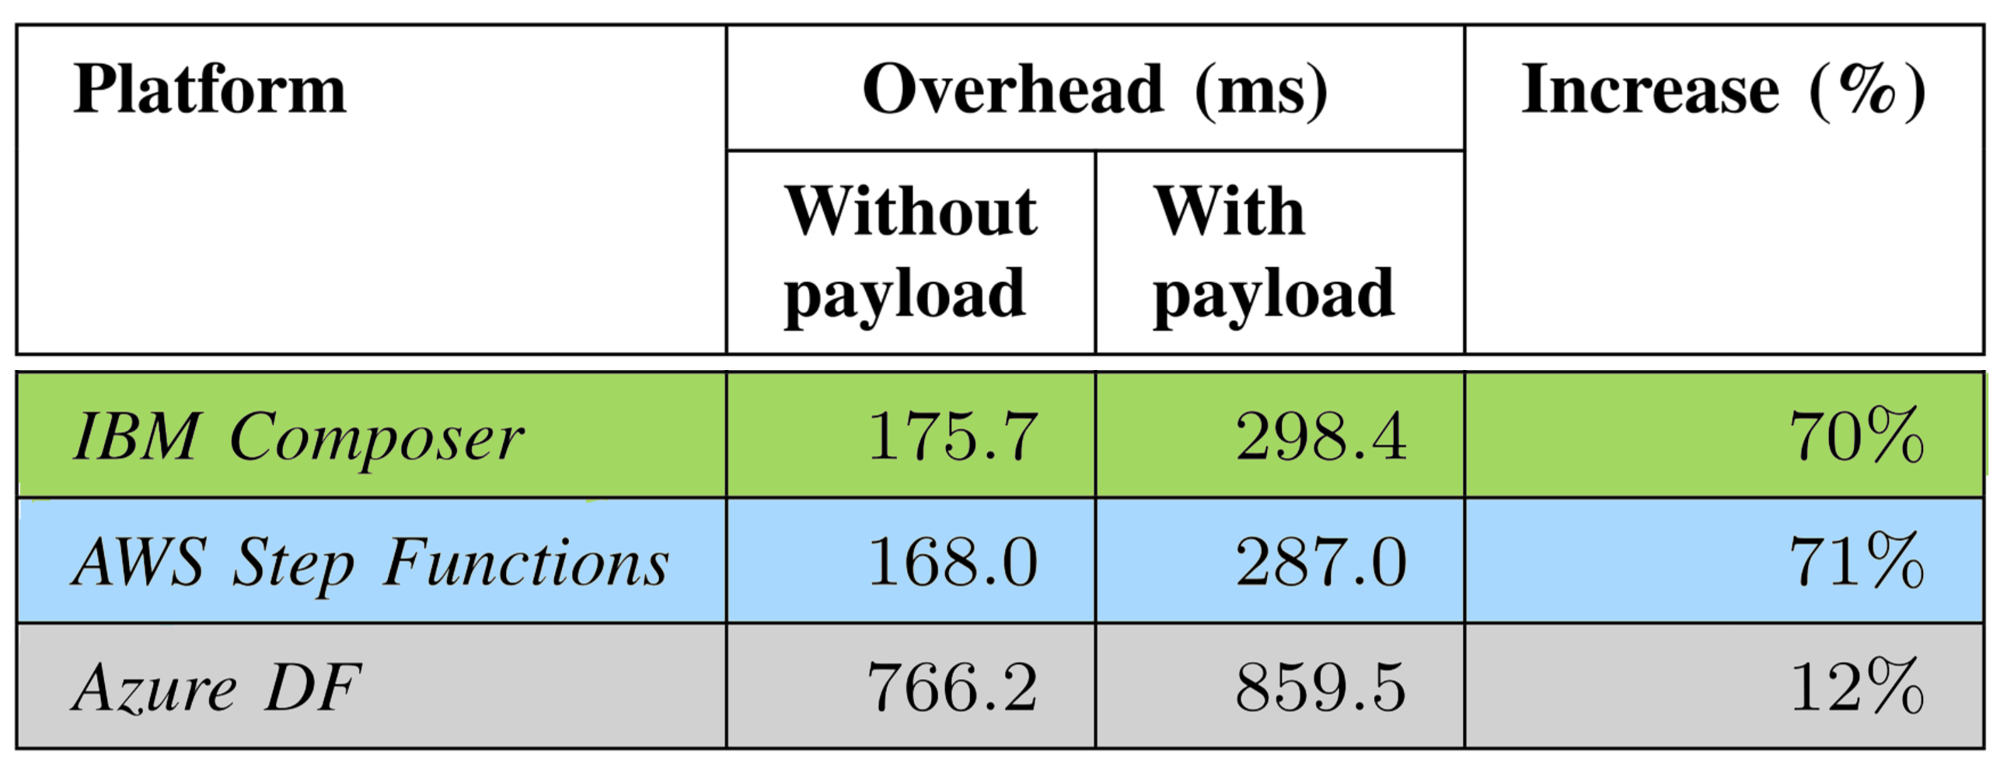
\includegraphics[width=0.7\textwidth]{Orchestration}
\end{figure} 
As shown by Lopez et al., AWS provides the most mature solution in terms of orchestration. Not only for sequential but also parallel execution AWS provides long-lived and short-lived function chaining. Also, the limitations on state transfer to 32KB enable AWS to provide clear information on pricing, compared with the other frameworks tested. When FaaS is mainly used for lightweight function chaining tasks, OpenWhisk in conjunction with IBM Composer is a suitable solution. With its limitation on chaining functions only up to 50 in number, OpenWhisk is slightly faster than AWS in that lower segment. For scheduling long-term running sequences, running for days or even month, OpenWhisk can not be recommended \cite{lopez2018comparison}. If the focus is on the exchange of large application states between functions and more significant latency can be accepted, Azure is capable of such a use case. By a capacity of 60KB it its by far ahead of its competitors. Even sequences that run for an extended period can be configured. Moreover using async/await syntax with sequential function chaining and fan-out/fan-in\footnote{https://docs.microsoft.com/en-us/azure/azure-functions/durable/durable-functions-cloud-backup} for parallel execution, simplifies development over solutions from AWS and IBM \cite{lopez2018comparison}.


\subsection{Selecting a suitable service}
The service for starting the migration should manifest specific characteristics. As mentioned above, and in section two, \textit{benefits and drawbacks}, there are a view things that need to be taken into account. Due to Javas CPU-intense runtime and the time for loading potentially large amounts of libraries, the language is likely to raise the time of cold starts, eventually resulting in higher latencies \cite{bardsley2018serverless}. Also, the object-oriented model of Java must be restructured to meet the requirements of the original functional programming style of FaaS. Concepts embraced by Java, such as getters, setters, empty methods, constructors, and singletons, need to be considered when mapping an object-oriented programming language to decoupled functional units.\\\\ Moreover, migrating from an object-oriented approach, respectively Java, state changes in classes and objects need to be treated separately. In a functional unit, keywords such as \textit{this}, referencing itself in a java-class, are not applicable. To address this issue, the self-reference, as suggested by Wright et al. \cite{wright1998compiling}, should be provided with the method signature. This way, the same underlying object structure can be equally invoked with every new instance of a function getting started. Operations on the container do not interfere with objects in other containers, and saving the state in external databases will not cause redundancy between the different objects \cite{spillner2017java}. Considering these additional steps of migrating a service, written in an object OOP language \cite{leitner2019mixed}, staring with one written in a functional programming language might be easier. The development team has to decide on the issue of refactoring in favour of rewriting. When the goal is to maintain consistency in language, accross the entire platform, the former decision is in favour. Otherwise, converting the service into a functional language, by rewriting it, could be another option. In the latter case, JavaScript, PHP, and Python, which primarily are functional, are suitable candidates for conversion.\\\\ Furthermore, the majority of practitioners use functional programming languages over OOP languages \cite{leitner2019mixed}, increasing the likelihood of finding solutions to problems on the internet. In contrast to legacy applications and the majority of PaaS and IaaS architectures, the service that is about to be converted should not experience consistently high loads. Services like the CI/CD pipeline, experiencing various workloads are suitable to be turned to FaaS. Besides that, looking at the existing microservice architecture and identifying services that spend most of their time in IDLE, can be considered for migration.


\subsection{Effects on teams, development and tooling}
When a microservice architecture is prevalent, FaaS can be adopted with fewer changes than a monolithic architecture \cite{fox2017status}. With FaaS, concepts like agile development, continuous delivery and continuous integration, as well as a different mindset amongst the development team, are probably more common. Nevertheless, FaaS goes a step further, then PaaS does, which suggests the assumption that the PaaS-adapted development structure will change. Starting with agile development and \glqq DevOps\grqq{}, Function as a Service forces companies and teams to adopt an agile mindset and agile techniques \cite{benlian2018transformative}. The necessity of iterative cycles is accounted for by the concepts of greater modularity compared to microservices. Persuing procedures form older waterfall driven projects are still prevalent, would not satisfy the core-features of Serverless, respectively, FaaS. With a significant reduction in lead time development, long periods of requirement engineering will hinder the effectiveness of FaaS. Teams that already incorporated agile process frameworks, such as scrum, will have an advantage over those remaining to acquire experience. Serverless development will enhance the importance of continuous delivery and continuous integration of integrating procedures like unit testing and integration testing, to diminish time to market to a minimum. Depending on the size and complexity, which should be kept to a minimum as well, the chances are that FaaS will be considerably faster than the current microservice development.\\\\ Furthermore, the size of the teams, to be more accurate, the number of developers working on a function, should experience a decrease. Whereas now two to three Developers are working on a microservice, separation of concerns, naturally imposed by FaaS, will further reduce complexity. Also, reducing complexity and focussing on a specific functionality can help to optimize each function further. By doing so, besides the reduction in startup latency, with the shorter execution time, the platform will charge less \cite{shafiei2020serverless}.\\\\ However, when maintaining a microservice infrastructure, each service and each version is likely to have a separate repository. With Function as a Service, this approach will be challenged regarding the number of functions that make up the application or service. Having a repository for each service, the odds are in favour of experiencing an overhead in version control, maintaining the landscape. Hence teams pursuing this approach are facing duplication in their code base, because the transparency of already existing functions, can not be gathered with little effort \cite{racicot2019quality}. This complexity and duplication seem to be the cause of why many users follow a mono-repository approach over having many small repositories \cite{brousse2019issue}.\\\\ With that said, FaaS seems to be conflicting with itself to some extent. Although its modularity suits the poly-repository approach quite well, the accompanying complexity, while an application keeps growing, can cause redundancy and inefficiency. Factors that influence the modifiability are the amount of duplicated code, the complexity of the code units and the coupling between the modules \cite{racicot2019quality}. As a suggestion, there should be a mono-repository-approach for each (scrum)-team and a ploy-repo approach for each division. Both would coexist with the VCS of the present microservice-architecture. This way, redundancy of code in a team is kept very low, by simultaneously having a manageable amount of repositories across a division of a company. With this approach, complexity can not be eliminated, but at least mitigated to a certain degree. Moreover, having different repositories for different teams in an organization will simplify the use of many accounts for development and testing, as discussed in a later section.\\\\ Literature is currently facing a lack of tooling, in terms of the variety and maturity provided [\cite{Yussupov2019_SystematicMappingStudyFaaS}, \cite{leitner2019mixed}]. With a share of around 80\% \cite{leitner2019mixed} of practitioners using the Serverless\footnote{https://serverless.com/} framework, this tool is the most frequently used in the market. Besides the Serverless Framework, Terraform\footnote{https://www.terraform.io/} and CloudFormation\footnote{https://aws.amazon.com/cloudformation/} are mentioned as well, but their appearance is far less to the former. Especially in conjunction with the CI/CD pipeline, the use of tooling can play an important role. By using one of the tools mentioned above, the deployment is configured withing those tools, providing an abstraction layer between the contemporary architecture and the provider's platform.Thereby these tools enable hybrid architectures across multiple cloud providers. Terraform and the Serverless Framework both manage resource configuration and therfore need to be connectd with the providers. The connection will be established depositing authentication data for all cloud solutions to be managed on the frameworks platfrom. By striving to gain independence and reduce the effect of vendor lock-in [see \textit{benefits and drawbacks}], these frameworks are supporting that process. Especially the Serverless Framework, thanks to its vast amount of plugins, provides, e.g. an offline simulation of AWS Lambda and the AWS Gateway.\\\\ Within this conjunction, additional operational tasks should not remain unmentioned. Even though Serverless, Terraform, and CloudFormation provide the opportunity to register many accounts from all kinds of serverless providers, including AWS, Azure, IBM and more, they face an initial load in configuration purposes. Another issue that needs to be addressed is that new features offered by a platform will not be adjusted to third parties, which engenders latency time until the third party might provide the feature. Thus, these IaC frameworks do not come for free\footnote{https://serverless.com/pricing/}. They can be used for free to a certain extent, but when it comes to more advanced tasks, they will charge the user. Finally, they do as well represent some vendor lock-in.\\\\ Depending on the purpose of multi-cloud solutions, there might be higher costs than using just one provider. If functions form one provider need to access another's providers function, its functions will be affected by cold starts. Moreover, the physical distance between the two data centres will affect latencies. If the primary purpose of deploying an application to different cloud providers is to have redundant systems in case one fails, the cost will not be affected too much. Still, additional operational tasks are required to guarantee a stable backup. Testing needs to be done not only on one but on all cloud providers, the application is mirrored to, which will cause additional costs besides the operational overhead of monitoring and testing.\\\\ Regarding the deployment pipeline, in practice, many tasks are handled via shell script or any other kind of scripts. Introducing serverless, special tooling for deploying a function to the desired platform is necessary and needs to be included in the existing pipeline. If not using one of the IaC frameworks mentioned above, the providers specific CLI has to be integrated, in the case of AWS Lambda CloudFormation. Integration can vary depending on the provider but is inevitable, according to practitioners \cite{ivanov2018implementation}.



\subsection{Testing}
There are several ways to test a serverless application. A distinction is made between local unit-testing, canary releases, as well as A/B testing and integration testing. While Openwhisk was the first framework offering local unit testing, the other provider has adopted this as well. Looking at AWS, Amazon provides with their open-source Serverless Application Model (SAM)\footnote{$https://aws.amazon.com/de/serverless/sam/?nc1=h_ls$} the possibility to build, test and debug the application locally. On Azure, Microsoft provides the so-called \textit{Function Core Tools} as integration for running functions locally\footnote{https://docs.microsoft.com/en-us/azure/azure-functions/functions-develop-local}. Even though the underlying business logic can be tested locally, there is no guarantee that the code will work the same when deploying the function into the actual ecosystem. A reason for that is the interaction with triggers, events, databases, functions and other services which, again, can not be simulated accordingly in a local environment. In contrast to that, hosting an application on-premise or via IaaS or PaaS, it is often possible to even simulate integration testing locally. Due to being in charge of the platform, there are often local copies on databases or message queues which are quite similar or identical to those running in production.\\\\ Moreover, it is hard to provide all configurations made on the different services locally. Key figures, such as the execution time of a function, the speed of loading all dependencies and potential latencies due to cold starts will be different on the cloud platform. Also, the unawareness on which type of server the function will be started in makes predictions on performance difficult \cite{racicot2019quality}. Due to the complexity being abstracted to the cloud vendor, the user has no further control over these services, then what the platform allows them to do. This restriction is not affected when performing unit tests, which is very easy, based on the small code base of the functions. With all these implications, it is inevitable to test the service on the provider's platform to get reliable results on compatibility and performance.\\\\ When testing on the platform, several possibilities can be chosen form. Starting with canary releases, considering the size of serverless functions, changing solely specific behaviour becomes far more feasible. After a new version is deployed, changes can be made to the API-Gateway of the serverless platform, in order to redirect a defined group of users, e.g. testers to the new version of the function or the entire application. Without being charged for code stored on the platform, only for code being run, it is possible to mirror the entire application to another account, without experiencing an increase in pricing. On that account, the new feature can be tested. Regarding the operational overhead of the mirroring process, mirroring appears to be more comparative on major changes to the application and or a function. For patches, solving defects, or minor changes, adding new features to a service not affecting is API mirroring might not be necessary. Using AWS, Azure or Google, canary releases can be scheduled via the CLI. On AWS in particular, canary releases can be achieved either via \textit{aws-lambda-deploy} or AWS Step Functions. Although the opportunity of canary releases and A/B testing theoretically exist, it is not very often used by operators \cite{leitner2019mixed}. One reason cloud be the operational overhead, another the implications on performance, when not having separate development and production accounts. Especially load tests are likely to affect performance on an account. In case only one account is used for testing and production, latencies can have a noticeable effect on the application, affecting end consumers. Therefore, it is advisable to have at least two different types of accounts — one for production and one for testing purposes. Despite the additional overhead, that way load tests can be done safely without any impact on the actual application \cite{leitner2019mixed}.



\subsection{Implications on monitoring}
Debugging and monitoring are crucial parts of any application. They ensure that the application is stable. The two metrics are indispensable in determining the health of an application during testing and later on in production. After going through the different testing environments, DEV, INT, UAT right up to PRD, the data gathered can be used as a baseline of the normal behaviour of a service. Whenever running out of memory or failing to provide a new instance of a service, the monitoring solution will, in a perfect world, alert the operator before issues in production cause severe damage. Whereas the team has full control over their servers when using a PaaS or IaaS solution, with a container environment like Kubernetes on top, it is quite different when switching to FaaS.
\begin{figure}[H]
\caption{Monitoring cloud functions, by \cite{manner2019troubleshooting}}
\label{fig:manner}
\centering
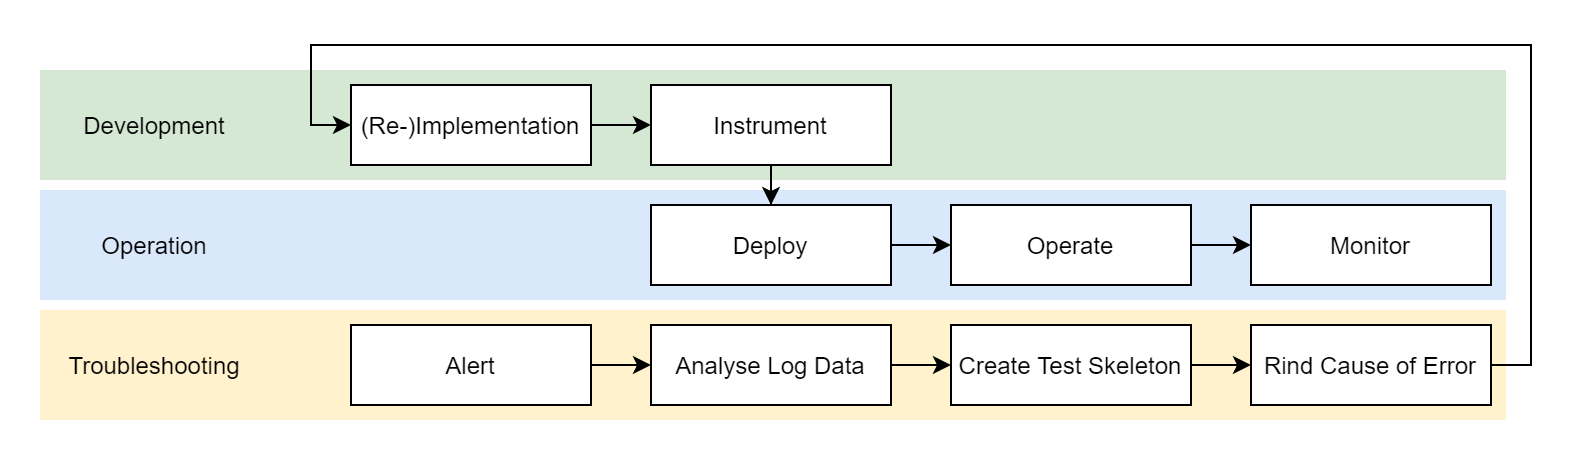
\includegraphics[width=1\textwidth]{monitoring}
\end{figure}
According to some papers [\cite{roberts2017serverless}, \cite{baldini2017serverless}], the field of serverless, mainly Functions as a Service, exhibits a lack of monitoring, logging and debugging solutions \cite{kritikos2018review}. Facing a lack of custom metrics, the operator solely relies on logging additional information needed, that are not provided by the platforms monitoring service. Not having access to the platforms infrastructure, is bound to the autonomy of the cloud provider for provisioning his platform. Enabling precise debugging on the environment would, as stated by \cite{manner2019troubleshooting}, take away the provider's control. Due to not having any control over the platform, it is crucial to monitor the functions constantly. In order to address this issue, Manner et al. provide monitoring and debugging approach. Because of its comprehensiveness, it will be recommended to be used for setting up a monitoring and debugging solution for cloud vendor platforms. For convenience only, figure ~\ref{fig:manner} shows the concept proposed by Manner et al. in a slightly modified way. The concept is split into three segments, namely development, operation and troubleshooting.\\\\ In the development-phase, the function should be implemented with three parameters that are going to be logged to an external database or monitoring service. These parameters are the input, the context and the output of the function which is being called. The limitation to three parameters is chosen, to not have too many repercussions on the execution time of the function. At the same time, the functions are providing enough data to reproduce failures when they occur \cite{manner2019troubleshooting}. After the functions have been tested on a development account, they will be forwarded to the production account. As a result of this, a clear distinction between the production and the development account is not necessary since they are identical. \\
In the second phase, the operational phase, the developer has to make use of monitoring services, which collect the data logged from each function. The received logging data will be further processed to determine a corridor for the execution times of a function. Whenever a function falls underneath a predefined execution time, an event will be triggered, which inform the ones in charge of operational purposes.\\ With an alert beeing send, the troubleshooting-phase is launched. In order to create a test skeleton consisting of the three logged parameters, all functions failed or exceeding the corridor, are filtered to retrieve their logging-data. Afterwards, the placeholders of the skeleton are replaced with the actual data to find the cause of the error \cite{manner2019troubleshooting}. This process will ideally be combined with the development account, not to affect the performance of the production account. At last, it is essential to log the date before the function returns a response asynchronously. After returning a response, the container will be discarded immediately stopping any processing.\\\\ Looking at open-source frameworks, it is crucial to be aware of the modularity which comes along with Function as a Service. When monitoring an environment, logging data from services and complementary parts will be collected. The data collected has to be stored within a database, being able to run aggregation, sorting and other types of evaluation metrics upon. Implementing an open-source FaaS framework into existing infrastructure, function monitoring can be included in the present monitoring solution. Being in charge of the infrastructure, metrics can be collected on a far deeper scale, e.g. the container runtime itself and as well as from the underlying OS. In case the former landscape consists of several more extensive services, potential bottlenecks need to be determined and have to be eliminated. The bottlenecks could occur in the form of connection pools to databases and need to be adjusted. With potentially many functions, that again have many instances; the connection pool has to scale dynamically. Another solution is a central message queue; all functions can provide their logging data to. As the message queue usually is faster than the database, it will collect the asynchronously logged data and forward it to the database.
\subsection{Summary}
\begin{figure}[H]
\caption{Modified DevOps pipeline}
\label{fig:devopsModified}
\centering
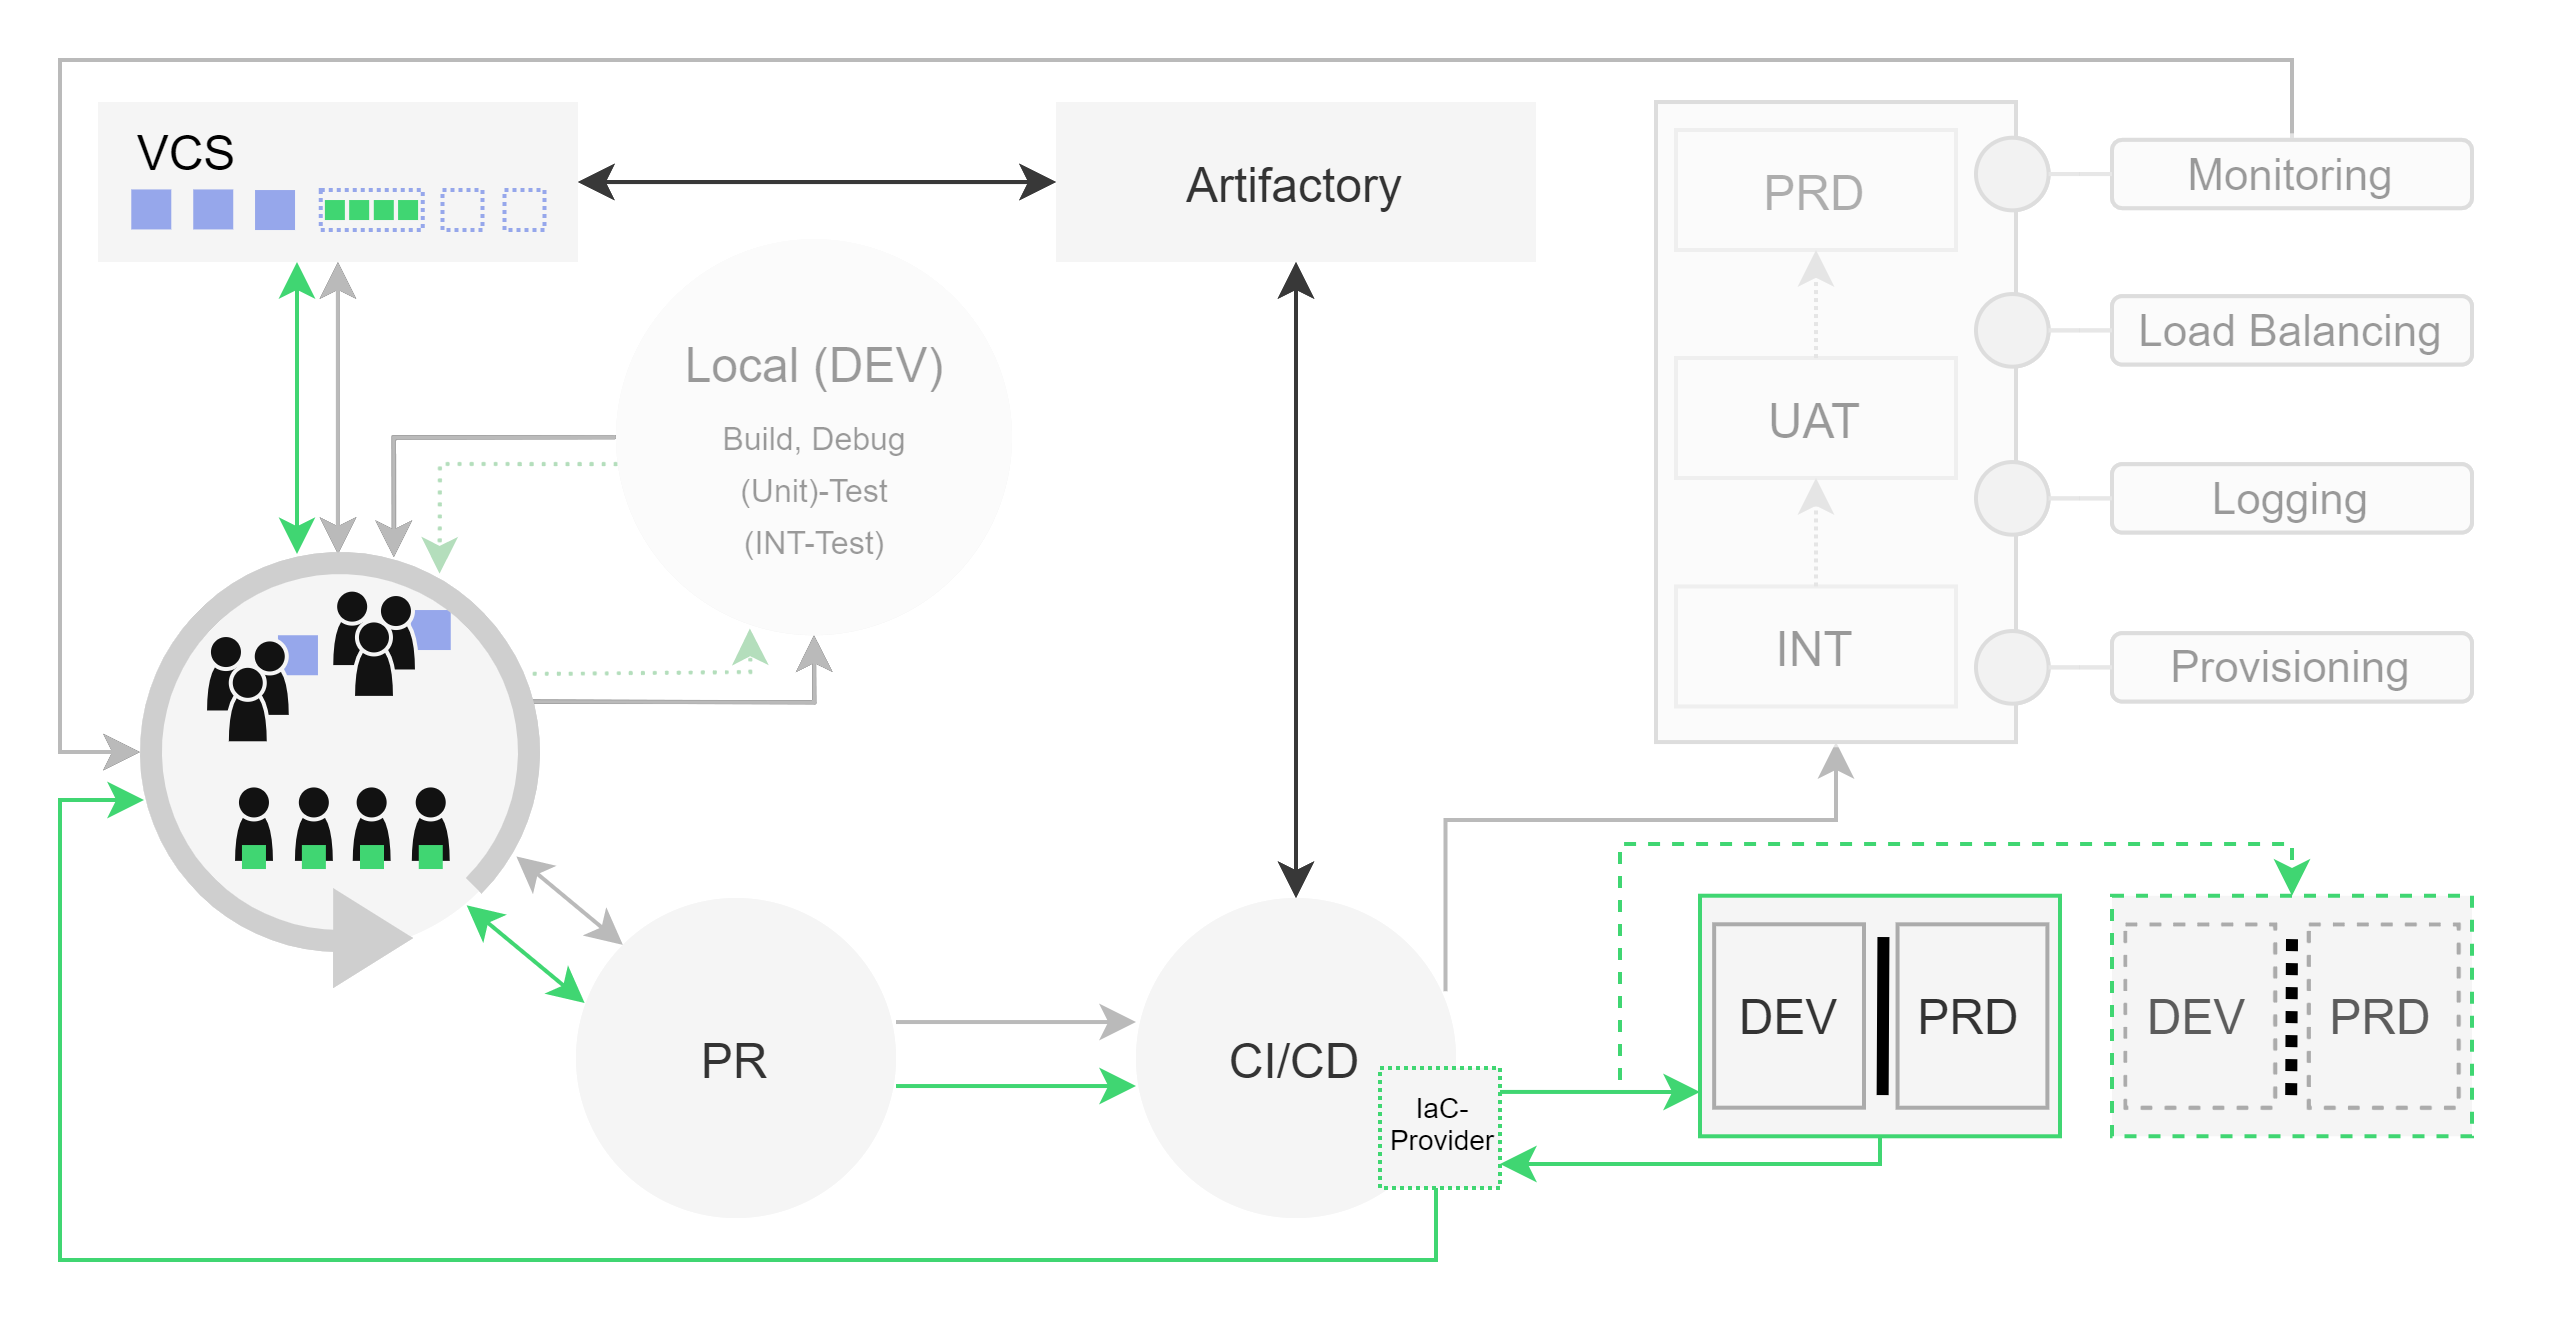
\includegraphics[width=1\textwidth]{DevOps modified}
\end{figure}
\newpage
\section{Anwendung des Leitfadens}
\subsection{Auswertung der Ergebnisse}
% INT UAT und Prod aus gutem Gund, aufgrundvon  e2e sowie lpts der verschiedenen Services. In finanysektor vor allem bei last tests ... lack of focus on  large scale enterprise applications \cite{kumar2019serverless}.
%Adopting serverless requires a different mental model, where systems are primarily constructed by composing pre-existing services, with FaaS often acting as the “glue” that brings these services together. FaaSofferstechnicalandbusiness-relatedadvantages, but managing and predicting deployment costs is difficult for larger applications. Further, tooling availability and maturity, especially related to testing and deployment, remains a barrier to entry. Finally, limited support for function sharing and the absence of a service ecosystem is seen as a challenge.  \cite{leitner2019mixed}
\subsubsection{Beurteilung der Kollaborationsauswirkungen}
\subsubsection{Beurteilung der Stabilität}
\subsubsection{Beurteilung der Skalierbarkeit} 
\subsubsection{Beurteilung des Monitorings}
\subsubsection{Beurteilung der Testmöglichkeiten} 
\subsection{Korrektur und Anpassungen}
\section{Abschließende Betrachtung}
\subsection{Absehbare Entwicklungen}
\cite{al2019systematic} Serverless  immer mehr bekanntheit und mehr Papers etc. ... Später market für funktionen die optimiert sind etc. \cite{shafiei2020serverless}\\
Real time communication tool  \cite{shafiei2020serverless} \\
Real time tracking gps  \cite{shafiei2020serverless} da beide nicht auf dem Application state benötigen/ beruhen  \cite{shafiei2020serverless} \\
\cite{hellerstein2018serverless}
\subsection{Zusammenfassung}
\subsection{Weiterführende Forschung}
Serverless Computing: A Survey of Opportunities, Challenges and Applications store for functions
\cite{shahrad2019architectural}
\newpage
\printbibliography%[title={Literaturverzeichnis}]
\end{document}